\AtBeginDocument{\paperdetails{
    submitted=2019-09-30,
    published=2020-02-17,
    year=2020,
    volume=4,
    issue=3,
    articlenumber=8,
  }}
\documentclass[english,crc,references=cleveref]{programming}
\usepackage[backend=biber]{biblatex}
\addbibresource{paper.bib}
% \usepackage{multicol}
% \usepackage{microtype}
% \usepackage{amssymb}
\usepackage{xypic}
\usepackage{semantic}
% \usepackage{amsmath}
\usepackage{amsthm}
% \usepackage{enumitem}

\AtBeginDocument{
  \newcounter{thc}
\newcounter{dfc}
\theoremstyle{plain}
\newtheorem{lem}[thc]{Lemma}
\newtheorem{theorem}[thc]{Theorem}

\theoremstyle{definition}
\newtheorem{axiom}[dfc]{Axiom}
\newtheorem{definition}[dfc]{Definition}
}

\definecolor{cmtclr}{rgb}{0.0,0.6,0.0}
\definecolor{kvdclr}{rgb}{0.0,0.0,0.6}
\definecolor{idclr}{rgb}{0.0,0.0,0.0}
\definecolor{numclr}{rgb}{0.0,0.4,0.0}
\definecolor{strclr}{rgb}{0.4,0.4,0.0}
\definecolor{rstrclr}{rgb}{0.5,0.1,0.0}
\definecolor{prepclr}{rgb}{0.6,0.0,0.2}
\newcommand{\vect}[1]{\langl #1 \rangl}
\newcommand{\langl}{\begin{picture}(4.5,7)
\put(1.1,2.5){\rotatebox{60}{\line(1,0){5.5}}}
\put(1.1,2.5){\rotatebox{300}{\line(1,0){5.5}}}
\end{picture}}
\newcommand{\rangl}{\begin{picture}(4.5,7)
\put(.9,2.5){\rotatebox{120}{\line(1,0){5.5}}}
\put(.9,2.5){\rotatebox{240}{\line(1,0){5.5}}}
\end{picture}}
\newcommand{\ball}[1]{\FPeval{\result}{clip(201+#1)}\textnormal{\ding{\result}}}
\newcommand{\lsep}{\;\;|\;\;}
% \newcommand{\Num}[1]{\textcolor{numclr}{#1}}
\newcommand{\Num}[1]{\num[color=numclr]{#1}}
\newcommand{\str}[1]{\textnormal{\textcolor{strclr}{\sffamily "#1"}}}
\newcommand{\rstr}[1]{\textnormal{\textcolor{rstrclr}{\sffamily "#1"}}}
\newcommand{\ident}[1]{\textnormal{\textcolor{idclr}{\sffamily #1}}}
\newcommand{\qident}[1]{\textnormal{\sffamily \textquotesingle #1\textquotesingle}}
\newcommand{\dom}{\ident{dom}}
\newcommand{\kvd}[1]{\textnormal{\textcolor{kvdclr}{\sffamily #1}}}

\newcommand{\bndclr}[1]{\textcolor{kvdclr}{#1}}
\newcommand{\bkndclr}[1]{\textcolor{prepclr}{#1}}
\newcommand{\blblclr}[1]{\textcolor{numclr}{#1}}
\newcommand{\bnd}[1]{\textnormal{\textcolor{kvdclr}{\sffamily #1}}}
\newcommand{\bknd}[1]{\textnormal{\textcolor{prepclr}{\sffamily #1}}}
\newcommand{\blbl}[1]{\textnormal{\textcolor{numclr}{\sffamily #1}}}
\newcommand{\narrow}[1]{\hspace{-0.6em}#1\hspace{-0.6em}}
\newcommand{\rname}[1]{{\sffamily(#1)}}
\newcommand{\ername}[1]{\vspace{0.75em}\rname{#1}\hspace{0.5em}}
\newcommand{\preview}[1]{\,\textnormal{\guillemotleft} #1\textnormal{\guillemotright}\,}

\begin{document}
\title{Foundations of a live data exploration environment}
%\titlerunning{Learning to live with errors}
\author[a,b]{Tomas Petricek}
\authorinfo{%
%
 % Tomas
  is a lecturer at University of Kent. He is working on making programming and data science
easier and more accessible. His research interests span a range of areas including theory of
programming languages, tools for data science as well as history and philosophy of programming.
%
Previously, he contributed to functional programming and the development of the F\# language and
type providers at Microsoft Research and obtained PhD from University of Cambridge for his work
on coeffects, a theory of context-aware programming languages. Along the way, he became interested
in understanding programming through the perspective of history and philosophy of science and wrote
papers about the evolution of programming concepts such as types and errors.
%
Contact him at \email{tomas@tomasp.net}.}
\affiliation[a]{University of Kent, UK}
\affiliation[b]{and The Alan Turing Institute, UK}
\keywords{Data exploration, live programming, data journalism, instant previews}
\paperdetails{
  perspective=sciencetheoretical,
  area={Programming environments},
}
% https://dl.acm.org/ccs/ccs.cfm and generate your Classification
\begin{CCSXML}
<ccs2012>
<concept>
<concept_id>10002951.10003227.10003351</concept_id>
<concept_desc>Information systems~Data mining</concept_desc>
<concept_significance>300</concept_significance>
</concept>
<concept>
<concept_id>10011007.10011006.10011041</concept_id>
<concept_desc>Software and its engineering~Compilers</concept_desc>
<concept_significance>300</concept_significance>
</concept>
<concept>
<concept_id>10003120.10003121.10003129</concept_id>
<concept_desc>Human-centered computing~Interactive systems and tools</concept_desc>
<concept_significance>300</concept_significance>
</concept>
</ccs2012>
\end{CCSXML}
\ccsdesc[300]{Human-centered computing~Interactive systems and tools}
\ccsdesc[300]{Information systems~Data mining}
\ccsdesc[300]{Software and its engineering~Compilers}
\maketitle

\begin{abstract}
%
% Context: What is the broad context of the work? What is the importance of the general research area?
A growing amount of code is written to explore and analyze data, often by data analysts
who do not have a traditional background in programming, for example by journalists.
%
% Inquiry: What problem or question does the paper address? How has this problem or question been addressed by others (if at all)?
The way such data anlysts write code is different from the way software engineers do so.
They use few abstractions, work interactively and rely heavily on external libraries.
We aim to capture this way of working and build a programming environment that makes data exploration
easier by providing instant live feedback.

% Approach: What was done that unveiled new knowledge?
We combine theoretical and applied approach. We present the \emph{data exploration calculus},
a formal language that captures the structure of code written by data analysts. We then
implement a data exploration environment that evaluates code instantly during editing and shows
previews of the results.
%
% Knowledge: What new facts were uncovered? If the research was not results oriented, what new capabilities are enabled by the work?
We formally describe an algorithm for providing instant previews for the data exploration calculus
that allows the user to modify code in an unrestricted way in a text editor. Supporting interactive
editing is tricky as any edit can change the structure of code and fully recomputing the output
would be too expensive.
%
% Grounding: What argument, feasibility proof, artifacts, or results and evaluation support this work?
We prove that our algorithm is correct and that it reuses previous results when updating previews
after a number of common code edit operations. We also illustrate the practicality of our approach
with an empirical evaluation and a case study.

% Importance: Why does this work matter?
As data analysis becomes an ever more important use of programming, research on programming languages
and tools needs to consider new kinds of programming workflows appropriate for those domains and
conceive new kinds of tools that can support them. The present paper is one step in this important direction.

\end{abstract}

% ==================================================================================================

\section{Introduction}
\label{sec:intro}
One of the aspects that make spreadsheets easier to use than other programming tools is their
liveness. When you change a cell in Excel, the whole spreadsheet updates instantly
and you immediately see new results, without having to explicitly trigger re-computation
and without having to wait for an extensive period of time.

An increasing number of programming environments aim to provide a live development experience
for standard programming languages, but doing this is not easy. Fully recomputing the whole program
after every keystroke is inefficient and calculating how a change in the source code changes the
result is extremely hard when the text editor allows arbitrary changes.
Consider the following snippet that gets the release years of the $10$ most expensive movies from a
data set \ident{movies}:
%
\begin{equation*}
\begin{array}{l}
\kvd{let}~\ident{top} =\ident{movies}.\ident{sortBy}(\lambda x \rightarrow x.\ident{getBudget}())\\
\qquad .\ident{take}(\Num{10}).\ident{map}(\lambda x \rightarrow x.\ident{getReleased()}.\ident{format}(\str{yyyy}))\\
\end{array}
\end{equation*}
%
A live programming environment computes and displays the list of years. Suppose that the programmer then
makes $\Num{10}$ a variable and changes the date format:
%
\begin{equation*}
\begin{array}{l}
\kvd{let}~\ident{count} = \Num{10}\\
\kvd{let}~\ident{top} = \ident{movies}.\ident{sortBy}(\lambda x \rightarrow x.\ident{getBudget}())\\
\qquad .\ident{take}(\ident{count}).\ident{map}(\lambda x \rightarrow x.\ident{getReleased()}.\ident{format}(\str{dd-mm-yyyy}))\\
\end{array}
\end{equation*}
%
Ideally, the live programming environment should understand the change, reuse a cached result of the
first two transformations (sorting and taking the first 10 elements) and only evaluate the
\ident{map} operation to differently format the release dates of top 10 movies. Our environment
does this for a simple data exploration language in an unrestricted text editor. We discuss related
work in \cref{sec:future}, but we briefly review the most important directions here, in
order to situate our contributions.


\subsection*{Contributions}
We present the design and implementation of a live programming environment for a simple data exploration
language that provides correct and efficient instant feedback, yet is integrated into an
ordinary text editor. Our key contributions are:

\begin{itemize}
\item We introduce the \emph{data exploration calculus} (\cref{sec:calculus}), a small formally
  tractable language for data exploration. The calculus is motivated by our review
  of how data analysts work (\cref{sec:background}) and makes it possible to write simple,
  transparent and reproducible data analyses.

\item A live programming environment does not operate in batch mode and so we cannot follow classic
  compiler literature. We capture the essence of such new perspective (\cref{sec:formal})
  and use it to build our \emph{instant preview} mechanism (\cref{sec:previews}) that evaluates
  code instantly during editing.

\item We prove that our instant preview mechanism is correct (\cref{sec:evaluation-correctness}) and that
  it reuses previously evaluated values when possible (\cref{sec:evaluation-reuse}). We
  illustrate the practicality of the mechanism using an empirical evaluation
  (\cref{sec:evaluation-empirical}) and a case study (\cref{sec:evaluation-case}).
\end{itemize}

% ==================================================================================================

\begin{figure}
  \begin{wide}
    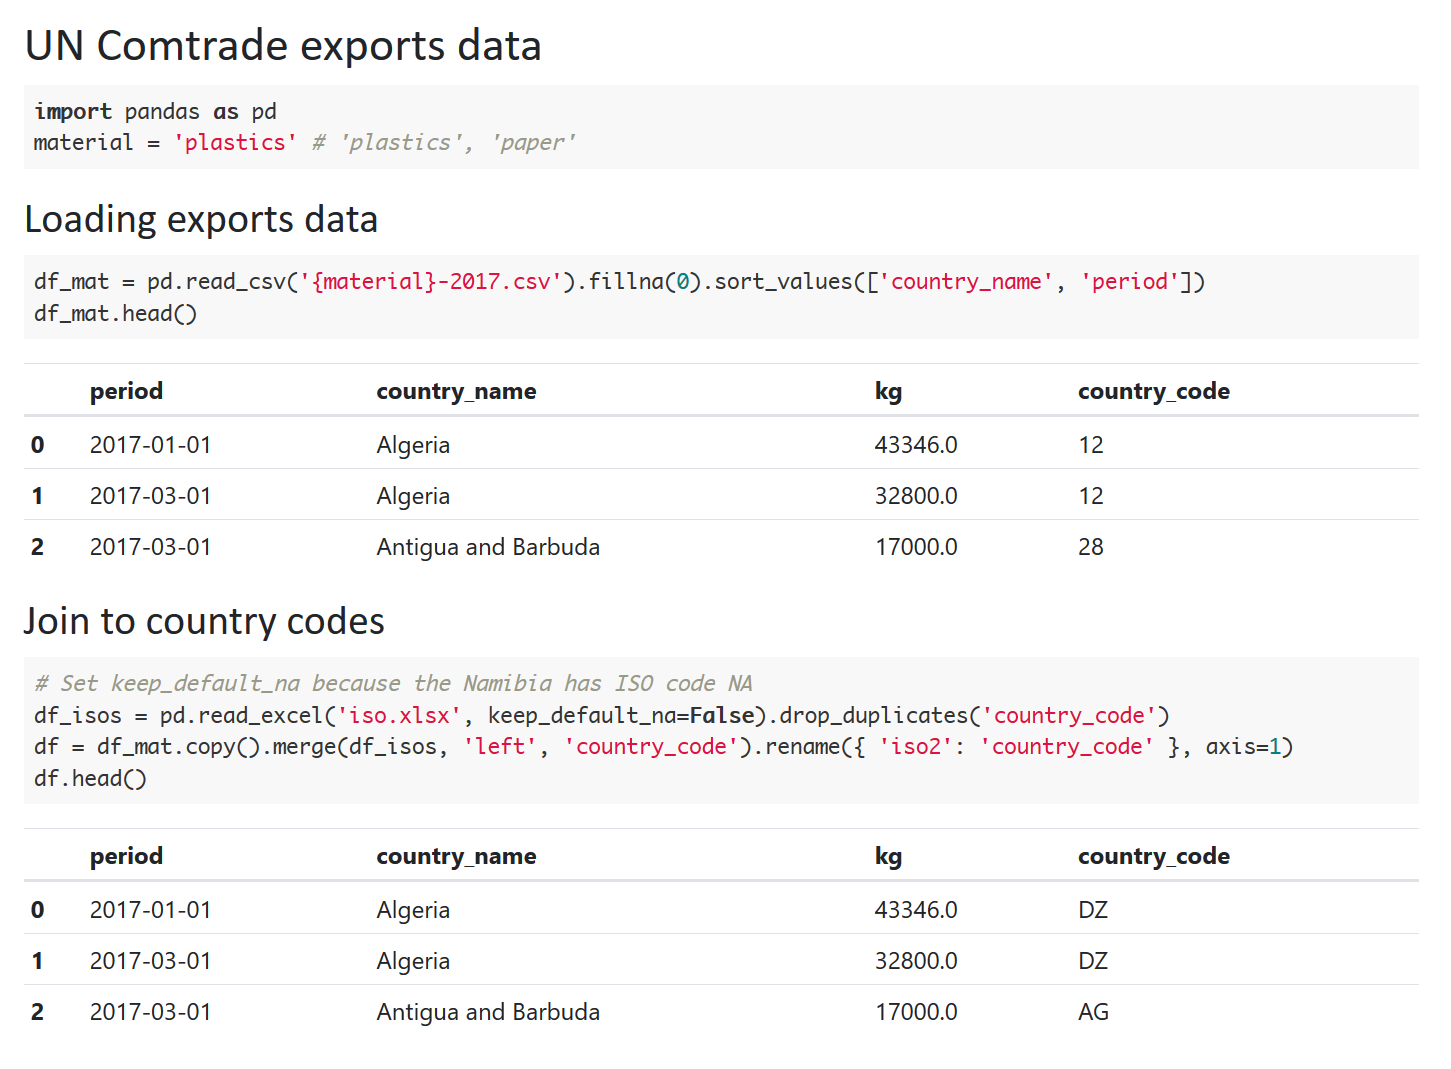
\includegraphics[width=\linewidth]{figures/notebook}
  \end{wide}
  \caption{Financial Times analysis that joins UN trade database with ISO country codes.}
\label{fig:ft-uncomtrade}
\end{figure}

% --------------------------------------------------------------------------------------------------

\section{Understanding how data scientists work}
\label{sec:background}

Data scientists often use general-purpose programming languages such as Python, but the kind of
code they write and the way they interact with the system is very different from how software
engineers work~\cite{workflow}. This paper focuses on simple data wrangling and data exploration as
done, for example, by journalists analysing government datasets. This new kind of non-expert
programmers is worth our attention as they often work on informing the public. They need easy-to-use
tools, but not necessarily a full programming langugae. In this section, we ilustrate how such
data analyses look and we provide a justification for the design of our data exploration calculus.

% --------------------------------------------------------------------------------------------------

\subsection{Simple data exploration in Jupyter}
\label{sec:background-jupyter}

Data analysts increasingly use notebook systems such as Jupyter, which make it possible to
combine text, equations and code with results of running the code, such as tables or visualizations.
Notebooks blur the conventional distinction between development and execution. Data analysts write
small snippets of code, run them to see results immediately and then revise them.

Notebooks are used by users ranging from scientists who implement complex models of physical
systems to journalists who perform simple data aggregations and create visualizations. Our
focus is on the simplest use cases. Making programmatic data exploration more
spreadsheet-like should encourage users to choose programming tools over spreadsheets, resulting
in more reproducible and transparent data analyses.

Consider the Financial Times analysis of plastic waste~\cite{ftnotebooks,ftarticle}. It joins
datasets from Eurostat, UN Comtrade and more, aggregates the data and
builds a visualization comparing waste flows in 2017 and 2018. \Cref{fig:ft-uncomtrade} shows
an excerpt from one notebook of the data analysis. The code has a number of important properties:
%
\begin{itemize}
%\vspace{0.5em}
\item There is no abstraction. The analysis uses lambda functions as arguments to library calls,
  but it does not define any custom functions. Code is parameterized by having a global variable
  \ident{material} set to \str{plastics} and keeping other possible values in a comment.
  This lets the analyst run and check results of intermediate steps.

%\vspace{0.5em}
\item The code relies on external libraries. Our example uses Pandas~\cite{pandas},
  which provides operations for data wrangling such as \ident{merge} to join datasets
  or \ident{drop\_duplicates} to delete rows with duplicate column values. Such standard libraries
  are external to the data analysis and are often implemented in another language like C++.

%\vspace{0.5em}
\item The code is structured as a sequence of commands. Some commands define a variable, either by
  loading data, or by transforming data loaded previously. Even in Python, data is often treated
  as immutable. Other commands produce an output that is displayed in the notebook.

%\vspace{0.5em}
\item There are many corner cases, such as the fact that \ident{keep\_default\_na}
  needs to be set to handle Namibia correctly. These are discovered interactively by
  running the code and examining the output, so providing an instant feedback is essential.
\end{itemize}
%
%\vspace{0.5em}
%
Many Jupyter notebooks are more complex than the above example and might use helper
functions or object-oriented code. However, simple data analyses such as the one discussed
here are frequent enough and pose interesting problems for programming tools.
This paper aims to bring such analyses to the attention of programming research community
by capturing their essential properties as a formal calculus.

% --------------------------------------------------------------------------------------------------

\begin{figure}
  \begin{wide}\centering
    \begin{subfigure}{.49\linewidth}
      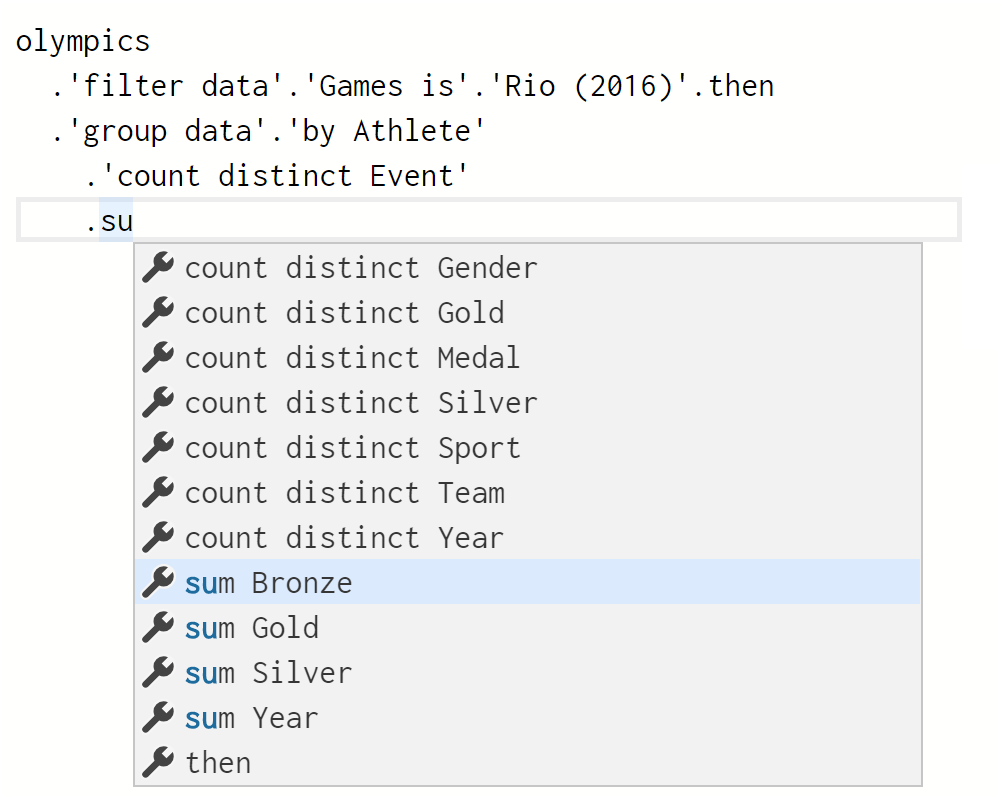
\includegraphics[width=\linewidth]{figures/gamma1.png}
      \caption{The analysis counts the number of distinct events per athlete.
        After typing `.' the editor offers further aggregation operations.}
  \label{fig:gamma-dot}
    \end{subfigure}\hfill
    \begin{subfigure}{.49\linewidth}
      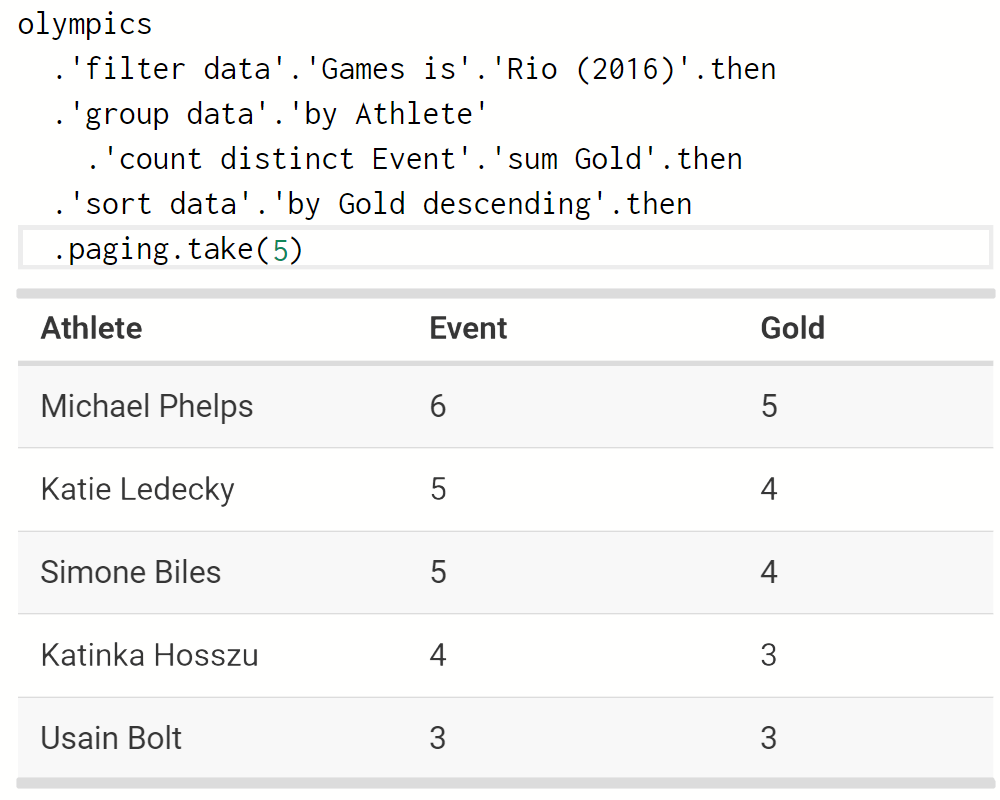
\includegraphics[width=\linewidth]{figures/gamma2.png}
      \caption{Our live programming environment for The Gamma. The table is
        updated on-the-fly and shows the result at the current cursor
        position.}
  \label{fig:gamma-preview}
    \end{subfigure}
  \end{wide}
% \vspace{0.5em}
\caption{Previous work on The Gamma with auto-complete based on type information (left)
  and our new editor with instant preview (right).}
\label{fig:gamma-intro}
\end{figure}

% --------------------------------------------------------------------------------------------------

\subsection{Dot-driven data exploration in The Gamma}
\label{sec:background-gamma}

\begin{sloppypar}
Simple data exploration has been the motivation for
a scripting language The Gamma~\cite{gamma}. Scripts in The Gamma are sequences of commands
that either define a variable or produce an output. It does not support top-level
functions and lambda functions can be used only as method arguments.
Given the limited expressiveness of The Gamma, libraries are implemented in other languages,
such as JavaScript. The Gamma uses type providers~\cite{providers-fsharp}
for accessing external data sources.
Type providers generate object types with members and The Gamma offers those in an
auto-complete list when the user types dot (`.') to access a member.
The combination of type providers and auto-complete makes it
possible to solve a large number of data exploration tasks through the very simple interaction of
selecting operations from a list.
\end{sloppypar}

The example in \cref{fig:gamma-dot} summarizes data on Olympic medals. Identifiers such
as \qident{sum Bronze} are names of members generated by the type provider. The type provider
used in this example generates an object with members for data transformations such as
\qident{group data}, which return further objects with members for specifying transformation
parameters, such as selecting the grouping key using \qident{by Athlete}.

The Gamma language is richer, but the example in \cref{fig:gamma-dot} shows that non-trivial
data exploration can be done using a very simple language. The assumptions about structure of
code that are explicit in The Gamma are implicitly present in Python and R data analyses
produced by journalists, economists and other users with other than programming background.
When we refer to The Gamma in this paper, readers not familiar with it can consider a small
subset of Python.

% --------------------------------------------------------------------------------------------------

\subsection{Live programming for data exploration}

The implementation that accompanies this paper builds a live programming environment for The Gamma.
It is discussed in \cref{sec:evaluation-case} and it replaces
the original text editor with just auto-complete with a live programming environment
that provides \emph{instant previews}.

An example of a instant preview is shown in \cref{fig:gamma-preview}. As noted earlier, The
Gamma programs consist of lists of commands which are either expressions or let bindings. Our
editor displays a instant preview below the command that the user is currently editing. The preview
shows the result of evaluating the expression or the value assigned to a bound variable. When the
user changes the code, the preview is updated automatically, without any additional interaction
with the user.

There are a number of guiding principles that inform our design. First, we allow the analyst
to edit code in an unrestricted form in a text editor. Although structured editors provide an
appealing alternative and make recomputation easier, we prefer the flexibility of plain text.
Second, we focus on the scenario when code changes, but input
does not. Rapid feedback allows the analyst to quickly adapt code to correctly handle
corner cases that typical analysis involves. In contrast to work on incremental computation,
we do not consider the case when data changes, although supporting interactive data exploration
of streaming data is an interesting future direction.

% ==================================================================================================

\section{Data exploration calculus}
\label{sec:calculus}

The \emph{data exploration calculus} is a small formal language for data exploration. The calculus
is not, in itself, Turing-complete and it can only be used together with external libraries that
define what objects are available and what the behaviour of their members is. This is
sufficient to capture the simple data analyses discussed in \cref{sec:background}. We
define the calculus in this section and then use it to formalise our instant preview
mechanism in \cref{sec:formal}.
%
The instant preview mechanism does not rely on types and so we postpone the discussion of static
typing to \cref{sec:extra-types}. Interestingly, it reuses the mechanism used for live
previews.

% --------------------------------------------------------------------------------------------------

\begin{figure}
\raggedright
\hspace{0.5em}{\sffamily Programs, commands, terms, expressions and values}
%
\begin{equation*}
\begin{array}{lcl}
p &\narrow{::=}& c_1; \ldots; c_n\\
c &\narrow{::=}& \kvd{let}~x = t \lsep t\\
\end{array}
\qquad
\begin{array}{lcl}
t &\narrow{::=}& o \lsep x \\
  &\narrow{|}& t.m(e, \ldots, e)
\end{array}
\qquad
\begin{array}{lcl}
e &\narrow{::=}& t \lsep \lambda x\rightarrow e\\
v &\narrow{::=}& o \lsep \lambda x\rightarrow e\\
\end{array}
\end{equation*}

%
\hspace{0.5em}{\sffamily Evaluation contexts of expressions}
%
\begin{equation*}
\begin{array}{lcl}
C_e[-] &=& C_e[-].m(e_1, \ldots, e_n) ~\lsep~ o.m(v_1, \ldots, v_{m}, C_e[-], e_1,\ldots , e_n) ~\lsep~ -\\
C_c[-] &=& \kvd{let}~x = C_e[-] ~\lsep~ C_e[-]\\
C_p[-] &=& o_1;\; \ldots;\; o_{k};\; C_c[-];\; c_{1};\; \ldots;\; c_n\\
\end{array}
\end{equation*}

%
\hspace{0.5em}{\sffamily Let elimination and member reduction}
%
\begin{equation*}
\begin{array}{ll}
\hspace{-0.5em}\begin{array}{l}
o_1;\; \ldots;\; o_{k};\; \kvd{let}~x=o;\; c_{1};\; \ldots; c_n \rightsquigarrow\\
\qquad  o_1;\; \ldots;\; o_{k};\; o; c_{1}[x\leftarrow o];\; \ldots; c_n[x\leftarrow o]\end{array} &
\quad\text{\rname{let}}\\[1.2em]
\inference
  {o.m(v_1, \ldots, v_n) \rightsquigarrow_\epsilon o'}
  {C_p[o.m(v_1, \ldots, v_n)] \rightsquigarrow C_p[o']} &
\quad\text{\rname{external}}
\end{array}
\end{equation*}

\caption{Syntax, contexts and reduction rules of the data exploration calculus}
\label{fig:dec-calculus}
\end{figure}

% --------------------------------------------------------------------------------------------------

\subsection{Language syntax}
The calculus combines object-oriented features such as member access with functional features
including lambda functions. The syntax is defined in \cref{fig:dec-calculus}. Object values
$o$ are defined by external libraries that are used in conjunction with the core calculus.

A program $p$ in the data exploration calculus consists of a sequence of commands~$c$. A command
can be either a let binding or a term. Let bindings define variables $x$ that can be used in
subsequent commands. Lambda functions
can only appear as arguments in method calls. A term $t$ can be a value, variable or a
member access, while an expression $e$, which can appear as an argument in member access,
can be a lambda function or a term.

%\footnote{Similar but weaker restrictions
%exist in other languages. To guide type inference, lambda functions
%in C\# can appear as either method arguments or assigned to an explicitly typed variable, but they
%cannot be assigned to an implicitly typed variable.}

\subsection{Operational semantics}
\label{sec:calculus-semantics}

The data exploration calculus is a call-by-value language. We model evaluation as a small-step
reduction $\rightsquigarrow$. Fully evaluating a program results in an irreducible sequence of
objects $o_1;\; \ldots;\; o_n$ (one object for each command, including let bindings) which can be
displayed as intermediate results of the data analysis. The operational semantics is parameterized
by a relation $\rightsquigarrow_\epsilon$ that models the functionality of the external libraries
used with the calculus and defines the reduction behaviour for member accesses. The relation has the
following form:
%
\begin{equation*}
o_1.m(v_1, \ldots, v_n) \rightsquigarrow_\epsilon o_2
\end{equation*}
%
Here, the operation $m$ is invoked on an object and takes values (objects or function values) as arguments.
The reduction always results in an object.
\Cref{fig:dec-calculus} defines the reduction rules in terms of $\rightsquigarrow_\epsilon$
and evaluation contexts; $C_e$ specifies left-to-right evaluation of arguments of a method call,
$C_c$ specifies evaluation of a command and $C_p$ defines left-to-right evaluation of a program.
The rule \rname{external} calls a method provided by an external library in a
call-by-value fashion; \rname{let} substitutes a value of an evaluated variable in
all subsequent commands and leaves the result in the list of commands.
Note that our semantics does not define how $\lambda$ applications are reduced. This is done by
external libraries, which will typically supply functions with arguments using standard $\beta$-reduction.
The behaviour is subject to constraints discussed next.

\subsection{Example external library}
\label{sec:calculus-example}

The data exploration calculus is not limited to the data exploration domain.
It can be used with external libraries for a wide range of other simple programming tasks, such as image
manipulation, as done in \cref{sec:evaluation-empirical}. However, we choose a name that reflects the
domain that motivated this paper. To illustrate how a definition of an external library looks,
consider the following simple data manipulation script:
%
\begin{equation*}
\begin{array}{l}
\kvd{let}~l = \ident{list}.\ident{range}(\Num{0}, \Num{10})\\
l.\ident{map}(\lambda x \rightarrow \ident{math}.\ident{mul}(x, \Num{10}))
\end{array}
\end{equation*}
%
An external library provides the \ident{list} and \ident{math} values with members
\ident{range}, \ident{map} and \ident{mul}. The objects of the external library consist of
numbers $n$, lists of objects $[o_1, \ldots, o_k]$ and failed computations $\bot$~\cite{gowrong}.
Next, the external library needs to define the $\rightsquigarrow_\epsilon$ relation that defines
the evaluation of member accesses. The following shows the rules for members of lists, assuming
the only supported member is \ident{map}:
%
\begin{equation*}
\begin{array}{l}
\\[-0.75em]
\inference
  {e[x \leftarrow n_i] \rightsquigarrow o_i \quad (\textit{for all $i\in 1\ldots k$})}
  {[ n_1, \ldots, n_k ].\ident{map}(\lambda x\rightarrow e) \rightsquigarrow_\epsilon [ o_1, \ldots, o_k ]}
\qquad
\inference
  {(\textit{otherwise})}
  {[ n_1, \ldots, n_k ].m(v_1, \ldots, v_n) \rightsquigarrow_\epsilon \bot}
\\[-0.75em]
~
\end{array}
\end{equation*}
%
When evaluating \ident{map}, we apply the provided function to all elements of the list using
standard $\beta$-reduction, defined recursively using $\rightsquigarrow$, and return a list with
resulting objects. The $\rightsquigarrow_\epsilon$ relation is defined on all member accesses,
but non-existent members reduce to the failed computation $\bot$.

\subsection{Properties}
The data exploration calculus has a number of desirable properties. Some of those require that the
relation $\rightsquigarrow_\epsilon$, which defines evaluation for external libraries, satisfies a
number of conditions. We discuss \emph{normalization} and \emph{let elimination} in this section.
Those two are particularly important as they will allow us to prove correctness of our method of
evaluating instant previews in \cref{sec:evaluation-correctness}.

\begin{definition}[Further reductions]
\label{def:further-red}
We define two additional reduction relations:
\begin{itemize}
\item We write $\rightsquigarrow^{*}$ for the reflexive, transitive closure of $\rightsquigarrow$
\item We write $\rightsquigarrow_\ident{let}$ for a call-by-name let binding elimination
  $c_1;\; \ldots;\; c_{k-1};\;$\\ $\kvd{let}~x=t;\; c_{k+1};\; \ldots; c_n ~\rightsquigarrow_\ident{let}~
  c_1;\; \ldots;\; c_{k-1};\; t; c_{k+1}[x\leftarrow t];\; \ldots; c_n[x\leftarrow t]$
\end{itemize}
\end{definition}
%
%
We say that two expressions
$e$ and $e'$ are \emph{observationally equivalent} if, for any context~$C$, the expressions $C[e]$ and
$C[e']$ reduce to the same value. Lambda functions $\lambda x\!\rightarrow\!2$ and
$\lambda x\!\rightarrow\!1\!+\!1$ are not equal, but they are observationally equivalent.
We require that external libraries satisfy two conditions. First, when a method is called with
observationally equivalent values as arguments, it should return the same value. Second, the
evaluation of $o.m(v_1,\ldots,v_n)$ should be defined for all $o, n$ and $v_i$.
The definition in \cref{sec:calculus-example} satisfies those by using standard
$\beta$-reduction for lambda functions and by reducing all invalid calls to the $\bot$ object.

\begin{definition}[External library]
\label{def:external}
An external library consists of a set of objects $O$ and a reduction relation
$\rightsquigarrow_\epsilon$ that satisfies the following two properties:
\begin{description}
\item [Totality] For all $o, m, i$ and all $v_1, \ldots, v_i$, there exists $o'$ such
  that $o.m(v_1, \ldots, v_i) \rightsquigarrow_\epsilon o'$.
\item[Compositionality] For observationally equivalent arguments, the reduction should always return
  the same object, i.\hairspace e.~given $e_0, e_1, \ldots, e_n$ and $e'_0, e'_1, \ldots, e'_n$ and $m$ such that
  $e_0.m(e_1, \ldots, e_n) \rightsquigarrow^{*} o$ and $e'_0.m(e'_1, \ldots, e'_n) \rightsquigarrow^{*} o'$ then
  if for any contexts $C_0, C_1, \ldots, C_n$ it holds that if $C_i[e_i] \rightsquigarrow^{*} o_i$ and
  $C_i[e'_i] \rightsquigarrow^{*} o_i$ for some $o_i$ then $o = o'$.
\end{description}
\end{definition}
%
%
Compositionality is essential for proving the correctness of our instant preview mechanism and
implies determinism of external libraries.
Totality allows us to prove normalization, i.\hairspace e.~all programs reduce to
a value -- although the resulting value may be an error value provided by the external library.

\begin{theorem}[Normalization]
\label{thm:normalization}
For all $p$, there exists $n, o_1, \ldots, o_n$ such that $p\rightsquigarrow^{*} o_1;\ldots;o_n$.
\end{theorem}
\begin{proof}
A program that is not a sequence of values can be reduced and reduction decreases the size of the
program. See \cref{sec:app-normalization} for more detail.
\end{proof}
%
%
Although the reduction rules \rname{let} and \rname{external} of the data exploration calculus
define an evaluation in a call-by-value order, eliminating let bindings in a call-by-name way
using the $\rightsquigarrow_\ident{let}$ reduction does not affect the result. This
simplifies our later proof of instant preview correctness in \cref{sec:evaluation-correctness}.

\begin{lem}[Let elimination for a program]
\label{thm:let-lang-elimination}
Given any program $p$ such that $p \rightsquigarrow^{*} o_1;\ldots;o_n$ for some $n$ and $o_1, \ldots, o_n$
then if $p \rightsquigarrow_\ident{let} p'$ for some $p'$ then also $p' \rightsquigarrow^{*} o_1;\ldots;o_n$.
\end{lem}
\begin{proof}
By constructing $p' \rightsquigarrow^{*} o_1;\ldots;o_n$ from
$p \rightsquigarrow^{*} o_1;\ldots;o_n$. See \cref{sec:let-lang-elimination}.
\end{proof}

% ==================================================================================================

\section{Formalising a live programming environment}
\label{sec:formal}

A naive way of providing instant previews during code editing would be to re-evaluate the code
after each change. This would be wasteful -- when writing code to explore data, most changes are
additive. To update a preview, we only need to evaluate newly added code. We describe an
efficient mechanism in this section.

% --------------------------------------------------------------------------------------------------

\subsection{Maintaining the dependency graph}
\label{sec:formal-deps}

The key idea behind our method is to maintain a dependency graph~\cite{dependencies} with
nodes representing individual operations of the computation that can be evaluated
to obtain a preview. Each time the program text is modified, we parse it afresh (using an
error-recovering parser) and bind the abstract syntax tree to the dependency graph.
When binding a new expression to the graph, we reuse previously created nodes as long as
they have the same structure and the same dependencies. For expressions that have a new
structure, we create new nodes.

The nodes of the graph serve as unique keys into a lookup table containing previously
evaluated parts of the program. When a preview is requested for an expression, we use the graph
node bound to the expression to find a preview. If a preview has not been evaluated, we force
the evaluation of all dependencies in the graph and then evaluate the operation represented by
the current node.

% --------------------------------------------------------------------------------------------------

\subsubsection{Elements of the graph}
The nodes of the graph represent individual operations of the computation. In our design, the nodes
are used as cache keys, so we attach a unique symbol $s$ to some of the nodes. That way, we can
create two unique nodes representing, for example, access to a member named \ident{take} which
differ in their dependencies.

The graph edges are labelled with labels indicating the kind of dependency. For
a method call, the labels are ``first argument'', ``second argument'' and so on. Writing
$s$ for symbols and $i$ for integers, nodes (vertices) $\bndclr{v}$ and edge labels $\blblclr{l}$
are defined as:
%
\begin{equation*}
\begin{array}{rcll}
\bndclr{v}&=&\bnd{val}(o) \lsep \bnd{var}(x)\lsep \bnd{mem}(m, s)\lsep \bnd{fun}(x, s)&\qquad(\textit{Vertices})\\
\blblclr{l}&=&\blbl{body} \lsep \blbl{arg}(i)&\qquad(\textit{Edge labels})\\
\end{array}
\end{equation*}
%
The \bnd{val} node represents a primitive value and contains the object itself. Two occurrences
of $\Num{10}$ in the source code will be represented by the same node. Member access \bnd{mem}
contains the member name, together with a unique symbol $s$ -- two member access nodes with
different dependencies will contain a different symbol. Dependencies of member access are labelled
with \blbl{arg} indicating the index of the argument ($0$~for the instance and $1,\ldots$ for the
arguments). Finally, nodes \bnd{fun} and \bnd{var} represent function values and variables
bound by $\lambda$ abstraction.

% --------------------------------------------------------------------------------------------------

\subsubsection{Example graph}
\cref{fig:dep-graph} illustrates how we build the
dependency graph. Node representing $\ident{take}(x)$ depends on the argument -- the
number $\Num{15}$ -- and the instance, which is a node representing $\ident{skip}(\Num{10})$.
This depends on the instance \ident{data} and the number $\Num{10}$. Note that variables
bound via \kvd{let} binding such as $x$ do not appear as $\bnd{var}$ nodes. The node using it
depends directly on the node representing the expression assigned to $x$.

After changing the value of $x$, we create a new graph. The dependencies of the node
$\bnd{mem}(\ident{skip}, s_0)$ are unchanged and so the symbol $s_0$ attached to the node remains
the same and previously computed previews can be reused. This part of the program is not recomputed.
The $\blbl{arg}(1)$ dependency of the \ident{take} call
changed and so we create a new node $\bnd{mem}(\ident{skip}, s_2)$ with a fresh symbol $s_2$.
The preview for this node is then computed as needed using the already known values of its
dependencies.

% --------------------------------------------------------------------------------------------------

\begin{figure}
\centering
\subcaptionbox{
  \raggedright
  Graph constructed from initial expression:
  $\kvd{let}~x = \Num{15}~\kvd{in}~\ident{data.skip}(\Num{10}).\ident{take}(x)$
  \label{fig:dep-graph-a}
}{
  $\xymatrix{
  \bnd{val}(\Num{10}) & \bnd{val}(\Num{15})\\
  \bnd{mem}(\ident{skip},s_0)\ar[d]_{\blbl{arg}(0)} \ar[u]^{\blbl{arg}(1)} &
  \bnd{mem}(\ident{take},s_1)\ar[l]_{\blbl{arg}(0)} \ar[u]_{\blbl{arg}(1)}\\
  \bnd{var}(\ident{data})
  }\qquad$
  \vspace{0.5em}
}
\hspace{1em}
\subcaptionbox{
  \raggedright
  Updated graph after changing $x$ to $10$:
  $\kvd{let}~x = \Num{10}~\kvd{in}~\ident{data.skip}(\Num{10}).\ident{take}(x)$
  \label{fig:dep-graph-b}
}{
  $\xymatrix{
  \bnd{val}(\Num{10})&\\
  \bnd{mem}(\ident{skip}, s_0)\ar[d]_{\blbl{arg}(0)} \ar[u]^{\blbl{arg}(1)} &
  \bnd{mem}(\ident{take}, s_2)\ar[l]_{\blbl{arg}(0)} \ar@/_/[lu]_{\blbl{arg}(1)}\\
  \bnd{var}(\ident{data})
}\qquad$
\vspace{0.5em}
}
\vspace{0.5em}
\caption{Dependency graphs formed by two steps of the live programming process. }
\label{fig:dep-graph}
\vspace{0.5em}
\end{figure}

% --------------------------------------------------------------------------------------------------

\subsubsection{Reusing graph nodes}
The binding process takes an expression and constructs a dependency graph.
It uses a lookup table to reuse previously created member access and function value nodes. The key
in the lookup table is formed by a node kind together with a list of dependencies. A node kind
includes the member or variable name; a lookup table $\Delta$ then maps a node kind with a list
of dependencies to a cached node:
%
\begin{equation*}
\begin{array}{ll}
\bkndclr{k}~::=~\bknd{fun}(x)~|~\bknd{mem}(m)&(\textit{Node kinds})\\[0.2em]
\Delta(\bkndclr{k}, [(\bndclr{v_1},\blblclr{l_1}), \ldots, (\bndclr{v_n},\blblclr{l_n})])  & (\textit{Lookup for a node})
\end{array}
\end{equation*}
%
The example on the second line looks for a node of a kind $\bkndclr{k}$ that has dependencies
$\bndclr{v_1}, \ldots, \bndclr{v_n}$ labelled with labels $\blblclr{l_1}, \ldots, \blblclr{l_n}$.
We write $\Delta(\bkndclr{k}, l)\!\downarrow$ when a value for a key is not defined.
When creating the graph in \cref{fig:dep-graph-b},
we perform the following lookups:
%
\begin{equation*}
\begin{array}{ll}
\Delta(\bknd{mem}(\ident{skip}), [(\bnd{var}(\ident{data}),\blbl{arg}(0)), (\bnd{val}(\Num{10}), \blbl{arg}(1))]) &\qquad(1)\\
\Delta(\bknd{mem}(\ident{take}), [(\bnd{mem}(\ident{skip}, s_0),\blbl{arg}(0)), (\bnd{val}(\Num{10}), \blbl{arg}(1))]) &\qquad(2)
\end{array}
\end{equation*}
%
First, we look for the \ident{skip} member access. The result is the $\bnd{mem}(\ident{skip}, s_0)$
known from the previous step. We then look for the \ident{take} member access. In the earlier
step, the argument of \ident{take} was $\Num{15}$ rather than $\Num{10}$ and so this lookup fails.
We then construct a new node $\bnd{mem}(\ident{take}, s_2)$ and later add it to the cache.

% --------------------------------------------------------------------------------------------------

\begin{figure*}
  \begin{wide}
    \begin{align}
&\ident{bind-expr}_{\Gamma, \Delta}(e_0.m(e_1, \ldots, e_n)) = \bndclr{v}, (\{\bndclr{v}\} \cup V_0 \cup \ldots \cup V_n, E \cup E_0 \cup \ldots \cup E_n) \\
&\quad \textnormal{when}~\bndclr{v_i}, (V_i, E_i) = \ident{bind-expr}_{\Gamma, \Delta}(e_i)
~\textnormal{and}~\bndclr{v} = \Delta(\bknd{mem}(m),[(\bndclr{v_0}, \blbl{arg}(0)), \ldots, (\bndclr{v_n}, \blbl{arg}(n))])\notag\\
&\quad \textnormal{let}~E = \{ (\bndclr{v}, \bndclr{v_0}, \blbl{arg}(0)), \ldots, (\bndclr{v}, \bndclr{v_n}, \blbl{arg}(n))\}\notag\\
%
&\ident{bind-expr}_{\Gamma, \Delta}(e_0.m(e_1, \ldots, e_n)) = \bndclr{v}, (\{\bndclr{v}\} \cup V_0 \cup \ldots \cup V_n, E \cup E_0 \cup \ldots \cup E_n)\\
&\quad \textnormal{when}~\bndclr{v_i}, (V_i, E_i) = \ident{bind-expr}_{\Gamma, \Delta}(e_i)
~\textnormal{and}~\Delta(\bknd{mem}(m),[(\bndclr{v_0}, \blbl{arg}(0)), \ldots, (\bndclr{v_n}, \blbl{arg}(n))])\!\downarrow\notag\\
&\quad \textnormal{let}~\bndclr{v} = \bnd{mem}(m, s), s~\textnormal{fresh}
~\textnormal{and}~E = \{ (\bndclr{v}, \bndclr{v_0}, \blbl{arg}(0)), \ldots, (\bndclr{v},\bndclr{v_n}, \blbl{arg}(n)) \}\notag\\
%
&\ident{bind-expr}_{\Gamma, \Delta}(\lambda x \rightarrow e) = \bndclr{v}, (\{\bndclr{v}\} \cup V, \{e\} \cup E)\\
&\quad \textnormal{when}~\Gamma_1 = \Gamma \cup \{ x, \bnd{var}(x) \}
~\textnormal{and}~\bndclr{v_0}, (V, E) = \ident{bind-expr}_{\Gamma_1, \Delta}(e)
~\textnormal{and}~\bndclr{v} = \Delta(\bknd{fun}(x),[(\bndclr{v_0}, \blbl{body})])\notag\\
&\quad \textnormal{let}~e = (\bndclr{v}, \bndclr{v_0}, \blbl{body})\notag\\
%
&\ident{bind-expr}_{\Gamma, \Delta}(\lambda x \rightarrow e) = \bndclr{v}, (\{\bndclr{v}\} \cup V, \{e\} \cup E)\\
&\quad \textnormal{when}~\Gamma_1 = \Gamma \cup \{ x, \bnd{var}(x) \}
~\textnormal{and}~\bndclr{v_0}, (V, E) = \ident{bind-expr}_{\Gamma_1, \Delta}(e)
~\textnormal{and}~\Delta(\bknd{fun}(x),[(\bndclr{v_0}, \blbl{body})])\!\downarrow\notag\\
&\quad \textnormal{let}~\bndclr{v} = \bnd{fun}(x, s), s~\textnormal{fresh}
~\textnormal{and}~e = (\bndclr{v},\bndclr{v_0},\blbl{body})\notag\\
%
&\ident{bind-expr}_{\Gamma, \Delta}(o) = \bnd{val}(o), (\{\bnd{val}(o) \}, \emptyset) \\
&\ident{bind-expr}_{\Gamma, \Delta}(x) = \bndclr{v}, (\{ \bndclr{v} \}, \emptyset)~\textnormal{when}~\bndclr{v} = \Gamma(x)
\end{align}
  \end{wide}
\caption{Binding rules that define a construction of a dependency graph for an expression.}
\label{fig:binding-rules-expr}
\end{figure*}

% --------------------------------------------------------------------------------------------------

\begin{figure*}
\begin{wide}
\begin{align}
&\ident{bind-prog}_{\Gamma, \Delta}(\kvd{let}~x=e; c_2; \ldots; c_n) = \bndclr{v_1};\ldots;\bndclr{v_n}, (\{\bndclr{v_1}\} \cup V \cup V_1, E \cup E_1)\\
&\quad \textnormal{let}~\bndclr{v_1}, (V_1,E_1) = \ident{bind-expr}_{\Gamma,\Delta}(e_1)~\textnormal{and}~\Gamma_1 = \Gamma \cup \{(x,\bndclr{v_1})\} \notag\\
&\quad \textnormal{and}~\bndclr{v_2}; \ldots; \bndclr{v_n}, (V, E) = \ident{bind-prog}_{\Gamma_1, \Delta}(c_2; \ldots; c_n)\notag\\
%
&\ident{bind-prog}_{\Gamma, \Delta}(e; c_2; \ldots; c_n) = \bndclr{v_1};\ldots;\bndclr{v_n}, (\{\bndclr{v_1}\} \cup V \cup V_1, E \cup E_1)\\
&\quad \textnormal{let}~\bndclr{v_1}, (V_1,E_1) = \ident{bind-expr}_{\Gamma,\Delta}(e)
~\textnormal{and}~\bndclr{v_2}; \ldots; \bndclr{v_n}, (V, E) = \ident{bind-prog}_{\Gamma_1, \Delta}(c_2; \ldots; c_n)\notag\\
%
&\ident{bind-prog}_{\Gamma, \Delta}([]) = [], (\emptyset, \emptyset)
\end{align}
\end{wide}
\caption{Binding rules that define a construction of a dependency graph for a program.}
\label{fig:binding-rules-prog}
%
\end{figure*}


% --------------------------------------------------------------------------------------------------

\subsection{Binding expressions to a graph}
\label{sec:formal-bind}

After parsing modified code, we update the dependency graph and link each node of the abstract
syntax tree to a node of the dependency graph. This process is called
binding and is defined by the \ident{bind-expr} function (\cref{fig:binding-rules-expr})
and \ident{bind-prog} function (\cref{fig:binding-rules-prog}). Both functions are
annotated with a lookup table $\Delta$ and a variable
context~$\Gamma$. The variable context is a map from variable names to dependency graph nodes and
is used for variables bound using \kvd{let} binding.

When invoked, $\ident{bind-expr}_{\Gamma,\Delta}(e)$ returns a node $\bndclr{v}$ that corresponds
to the expression~$e$, paired with a dependency graph $(V, E)$ formed by nodes $V$ and labelled
edges $E$. That edges are written as $(\bndclr{v_1}, \bndclr{v_2}, \blblclr{l})$ and include a
label $\blblclr{l}$. The $\ident{bind-prog}_{\Gamma,\Delta}$ function works similarly, but turns
a sequence of commands into a sequence of nodes.

When binding a member access, we use \ident{bind-expr} recursively
to get a node and a dependency graph for each sub-expression. The nodes representing sub-expressions are
then used for lookup into $\Delta$, together with their labels. If a node already
exists in $\Delta$ it is reused (1). Alternatively, we create a new node containing a fresh symbol~(2).
%
The graph node bound to a function depends on a synthetic node $\bnd{var}(x)$ that represents a
variable of unknown value. When binding a function, we create a variable node and add it
to the variable context $\Gamma_1$ before binding the body. As with member access, the node
representing a function may (3) or may not (4) already exist in the lookup table.

When binding a program, we bind the first command and
recursively process remaining commands (9). For \kvd{let} binding (7), we bind the expression $e$
assigned to the variable to obtain a graph node $\bndclr{v_1}$. We then store the node in the
variable context $\Gamma_1$ and bind the remaining commands. The variable context is used
when binding a variable in \ident{bind-expr} (6) and so all variables declared using \kvd{let}
will be bound to a graph node representing the value assigned to the variable. When the command
is just an expression (8), we bind the expression using \ident{bind-expr}.

% --------------------------------------------------------------------------------------------------

\begin{figure}
%
\begin{equation*}
\begin{array}{l}
\ident{update}_{V,E}(\Delta_{i-1}) = \Delta_i~\textnormal{such that:}
\\
\quad\Delta_{i}(\bknd{mem}(m), [(\bndclr{v_0},\blbl{arg}(0)),\ldots, (\bndclr{v_n},\blbl{arg}(n))]) = \bnd{mem}(m, s)\\
\quad\quad \textnormal{when}~\bnd{mem}(m, s) \in V
~\textnormal{and}~(\bnd{mem}(m, s), \bndclr{v_i}, \blbl{arg}(i)) \in E~\textnormal{for}~i\in 0,..,n
\\
\quad\Delta_{i}(\bknd{fun}(x), [(\bndclr{v_1},\blbl{body})]) = \bnd{fun}(x, s)\\
\quad\quad \textnormal{when}~\bnd{fun}(x, s) \in V
~\textnormal{and}~(\bnd{fun}(x, s), \bndclr{v_1}, \blbl{body}) \in E
\\
\quad\Delta_{i}(\bkndclr{v}) = \Delta_{i-1}(\bkndclr{v})\quad \textnormal{(otherwise)}
\end{array}
\end{equation*}
%
\caption{Updating the node cache after binding a new graph}
\label{fig:loop}
%
\end{figure}

% --------------------------------------------------------------------------------------------------

\subsection{Edit and rebind loop}

During editing, the dependency graph is repeatedly updated according to the binding rules.
We maintain a series of lookup table states $\Delta_0, \Delta_1, \Delta_2, \ldots$ The initial
lookup table is empty, i.\hairspace e.~$\Delta_0 = \emptyset$. At a step $i$, we parse a program $p_i$
and obtain a new dependency graph using the previous $\Delta$. The result is
a sequence of nodes corresponding to commands of the program and a graph $(V, E)$:
%
\begin{equation*}
\bndclr{v_1}; \ldots; \bndclr{v_n}, (V, E) = \ident{bind-prog}_{\emptyset, \Delta_{i-1}}(p_i)
\end{equation*}
%
The new state of the cache is computed using $\ident{update}_{V, E}(\Delta_{i-1})$
defined in \cref{fig:loop}. The function adds newly created nodes from the graph
$(V, E)$ to the previous cache $\Delta_{i-1}$ and returns a new cache $\Delta_{i}$.

% ==================================================================================================

\section{Computing instant previews}
\label{sec:previews}

The binding process constructs a dependency graph after code changes. The nodes in the dependency
graph correspond to individual operations that will be performed when running the program. When
evaluating a preview, we attach partial results to nodes of the graph. Since the binding process
reuses nodes, previews for sub-expressions attached to graph nodes will also be reused.

In this section, we describe how previews are evaluated. The evaluation is done over the dependency
graph, rather than over the structure of program expressions as in the operational semantics
given in \cref{sec:calculus-semantics}. In \cref{sec:evaluation}, we prove that
resulting previews are the same as the result we would get by directly evaluating code and we
also show that no recomputation occurs when code is edited in certain ways.

% --------------------------------------------------------------------------------------------------

\subsection{Previews and delayed previews}

Programs in the data exploration calculus consist of sequence of commands. Those are
evaluated to a value with a preview that can be displayed to the user. However, we also support
previews for sub-expressions. This can be problematic if the current sub-expression is inside
the body of a function. For example:
%
\begin{equation*}
\begin{array}{l}
\kvd{let}~\ident{top} = \ident{movies}.\ident{take}(\Num{10}).\ident{map}(\lambda x \rightarrow x.\ident{getReleased}().\ident{format}(\str{dd-mm-yyyy}))
\end{array}
\end{equation*}
%
Here, we can directly evaluate sub-expressions \ident{movies} and $\ident{movies}.\ident{take}(\Num{10})$,
but not $x.\ident{getReleased}()$ because it contains a free variable $x$. Our preview evaluation algorithm addresses this by
producing two kinds of previews. A \emph{fully evaluated preview} is just a value, while
a \emph{delayed preview} is a partially evaluated expression with free variables:
%
\begin{equation*}
\begin{array}{rcll}
p&=&o \lsep  \lambda x\rightarrow e&\quad(\textit{Fully evaluated previews})\\
d&=&p \lsep  \llbracket e \rrbracket_\Gamma&\quad(\textit{Evaluated and delayed previews})\\
\end{array}
\end{equation*}
%
A fully evaluated preview $p$ can be either a primitive object or a function value with no free
variables. A possibly delayed preview $d$ can be either an evaluated preview $p$ or an expression
$e$ that requires variables $\Gamma$. We use an untyped language and so $\Gamma$ is just a list of
variables $x_1, \ldots, x_n$. As discussed in \cref{sec:app-theories},
delayed previews have an interesting theoretical link with graded comonads.
The body of a lambda function may have a fully evaluated preview if it uses only variables that
are bound by earlier let bindings, but it will typically be delayed. We consider a speculative
design for an abstraction mechanism that better supports instant previews in
\cref{sec:extra-abstraction}.

% --------------------------------------------------------------------------------------------------

\begin{figure*}
\begin{equation*}
%
\hspace{-0.5em}
\begin{array}{l}
\inference[\rname{lift-expr}~]
  {\bndclr{v} \Downarrow \llbracket e \rrbracket_\Gamma}
  {\bndclr{v} \Downarrow_{\ident{lift}} \llbracket e \rrbracket_\Gamma}
\\
\\
\inference[\rname{lift-prev}~]
  {\bndclr{v} \Downarrow p}
  {\bndclr{v} \Downarrow_{\ident{lift}} \llbracket p \rrbracket_\emptyset}
\\
\\
\inference[\rname{val}~]
  {~}
  {\bnd{val}(o) \Downarrow o }
\\
\\
\inference[\rname{var}~]
  {~}
  {\bnd{var}(x) \Downarrow \llbracket x \rrbracket_x}
  \\[0.5em]~
\end{array}
\qquad\quad
\begin{array}{l}
\inference[\rname{fun-val}~]
  { (\bnd{fun}(x, s), \bndclr{v}, \blbl{body}) \in E & \bndclr{v} \Downarrow p }
  { \bnd{fun}(x, s) \Downarrow \lambda x\rightarrow p }
\\
\\
\inference[\rname{fun-bind}~]
  { (\bnd{fun}(x, s), \bndclr{v}, \blbl{body}) \in E & \bndclr{v} \Downarrow \llbracket e \rrbracket_{x} }
  { \bnd{fun}(x, s) \Downarrow \lambda x\rightarrow e }
\\
\\
\inference[\rname{fun-expr}~]
  { (\bnd{fun}(x, s), \bndclr{v}, \blbl{body}) \in E & \bndclr{v} \Downarrow \llbracket e \rrbracket_{x,\Gamma} }
  { \bnd{fun}(x, s) \Downarrow \llbracket \lambda x\rightarrow e \rrbracket_\Gamma }
\\[0.5em]~
\end{array}
\end{equation*}
%
\begin{equation*}
\hspace{-1em}
\begin{array}{l}
\inference[\rname{mem-val}~]
  { \forall i\in\{0\ldots k\}.(\bnd{mem}(m, s), \bndclr{v_i}, \blbl{arg}(i)) \in E & \bndclr{v_i} \Downarrow p_i
    & p_0.m(p_1, \ldots, p_k) \rightsquigarrow_\epsilon p }
  { \bnd{mem}(m, s) \Downarrow p }
\\
\\
\inference[\rname{mem-expr}~]
  { \forall i\in\{0\ldots k\}.(\bnd{mem}(m, s), \bndclr{v_i}, \blbl{arg}(i)) \in E & \exists j\in\{0\ldots k\}.\bndclr{v_j}\diagup\hspace{-1em}\Downarrow p_j
   & \bndclr{v_i} \Downarrow_{\ident{lift}} \llbracket e_i \rrbracket_{\Gamma_i}  }
  { \bnd{mem}(m, s) \Downarrow \llbracket e_0.m(e_1, \ldots, e_k) \rrbracket_{\Gamma_0,\ldots,\Gamma k} }
\\
\end{array}
\end{equation*}
\caption{Rules that define evaluation of previews over a dependency graph for a program}
\label{fig:eval}
\end{figure*}

% --------------------------------------------------------------------------------------------------

\subsection{Evaluation of previews}
The evaluation of previews is defined in \cref{fig:eval}. Given a dependency graph $(V, E)$,
the relation $\bndclr{v}\Downarrow d$ evaluates a sub-expression corresponding to
the node $\bndclr{v}$ to a possibly delayed preview $d$. The nodes $V$ and edges $E$ of the
graph are parameters of $\Downarrow$, but they do not change during the
evaluation and so we do not explicitly write them.

The auxiliary relation $\bndclr{v}\Downarrow_{\ident{lift}} d$ always evaluates
to a delayed preview. If the ordinary evaluation returns a delayed preview, so does the auxiliary
relation \rname{lift-expr}. If the ordinary evaluation returns a value, the value is wrapped
into a delayed preview requiring no variables \rname{lift-prev}.
%
A node representing a value is evaluated to a value \rname{val} and a node representing
an unbound variable is reduced to a delayed preview that requires the variable and returns its
value~\rname{var}.

For member access, we distinguish two cases. If all arguments evaluate to values \rname{member-val},
then we use the evaluation relation defined by external libraries $\rightsquigarrow_\epsilon$ to
immediately evaluate the member access and produce a value. If some of the arguments are
delayed \rname{member-expr}, because the member access is inside the body of a lambda function,
we produce a delayed member access expression that requires the union of the variables
required by the individual arguments.

The evaluation of function values is similar, but requires three cases. If the body can
be reduced to a value with no unbound variables \rname{fun-val}, we return a lambda function that
returns the value. If the body requires only the bound variable \rname{fun-bind}, we return a
lambda function with the delayed preview as the body. If the body requires further variables,
the result is a delayed preview.

\subsection{Caching of evaluated previews}
\label{sec:previews-cache}

For simplicity, the relation $\Downarrow$ in \cref{fig:eval} does not specify how previews
are cached. In practice, this is done by maintaining a lookup table from graph nodes $\bndclr{v}$
to previews $p$. Whenever $\Downarrow$ is used to obtain a preview for a graph node, we first
check the lookup table. If the preview has not been previously evaluated, we evaluate it and add
it to the lookup. Cached previews can be reused in two ways. First, if the same sub-expression
appears multiple times in the program, it will share a graph node and the preview will be resued.
Second, when binding modified source code, the process reuses graph nodes and so previews are
also reused during code editing.

% ==================================================================================================

\section{Evaluating live programming environment}
\label{sec:evaluation}

Computing previews using a dependency graph implements a correct and efficient optimization.
In this section we show that this is the case, first theoretically in \cref{sec:evaluation-reuse},
and then empirically in \cref{sec:evaluation-empirical}. We also describe a case study where
we developed an online service for data exploration based on the methods discussed in this paper
(\cref{sec:evaluation-case}).

% --------------------------------------------------------------------------------------------------

\subsection{Correctness of previews}
\label{sec:evaluation-correctness}

To show that the previews are correct, we prove two properties. Correctness (\cref{thm:correcntess})
guarantees that, the previews we calculate using a dependency graph are the same as the values we
would obtain by evaluating the program directly. Determinacy (\cref{thm:determinacy})
guarantees that previews assigned to a graph node based on an earlier graph are the same as
previews that we would obtain afres using an updated graph.

To simplify the proofs, we consider programs without let bindings. Eliminating let bindings does
not change the result of evaluation, as shown in \cref{thm:let-lang-elimination}, and it also
does not change the constructed dependency graph as shown below in \cref{thm:let-grp-elimination}.

\begin{lem}[Let elimintion for a dependency graph]
\label{thm:let-grp-elimination}
Given programs $p_1, p_2$ such that $p_1 \rightsquigarrow_\ident{let} p_2$ and a lookup table
$\Delta_0$ then if $\bndclr{v_1}; \ldots; \bndclr{v_n}, (V, E) = \ident{bind-prog}_{\emptyset, \Delta_0}(p_1)$ and
$\bndclr{v'_1};\ldots;\bndclr{v'_n}, (V', E') = \ident{bind-prog}_{\emptyset, \Delta_1}(p_2)$ such that $\Delta_1 = \ident{update}_{V, E}(\Delta_0)$
then for all $i$, $\bndclr{v_i} = \bndclr{v'_i}$ and also $(V, E) = (V', E')$.
\end{lem}
\begin{proof}
By analysis of the binding process. See \cref{sec:app-let-grp-elimination}.
\end{proof}
%
%
The \cref{thm:let-grp-elimination} provides a way of removing let bindings from a program,
such that the resulting dependency graph remains the same. Here, we bind the original program
first, which adds the node for $e$ to $\Delta$. In our implementation, this is not needed
because $\Delta$ is updated while the graph is being constructed using $\ident{bind-expr}$.
To keep the formalisation simpler, we separate the process of building the dependency graph
and updating $\Delta$ and thus \cref{thm:let-grp-elimination} requires an extra binding step.

Now, we can show that, given a let-free expression, the preview obtained using a correctly
constructed dependency graph is the same as the one we would obtain by directly evaluating the
expression. This requires a simple auxiliary lemma.

\begin{lem}[Lookup inversion]
\label{thm:lemma-lookup}
Given $\Delta$ obtained using \ident{update} in \cref{fig:loop} then:
\begin{itemize}
\raggedright
\item If $\bndclr{v}=\Delta(\bknd{fun}(x),[(\bndclr{v_0}, \blblclr{l_0})])$
then $\bndclr{v}=\bnd{fun}(x, s)$ for some $s$.
\item If $\bndclr{v}=\Delta(\bknd{mem}(m),[(\bndclr{v_0}, \blblclr{l_0}), \ldots, (\bndclr{v_n}, \blblclr{l_n})])$
then $\bndclr{v}=\bnd{mem}(m, s)$ for some $s$.
\end{itemize}
\end{lem}
\begin{proof}
By construction of $\Delta$ in \cref{fig:loop}.
\end{proof}

\begin{theorem}[Term preview correctness]
\label{thm:let-free-correct}
Given a term $t$ that has no free variables, together with a lookup table $\Delta$ obtained
from any sequence of programs using $\ident{bind-prog}$ (\cref{fig:binding-rules-prog}) and
$\ident{update}$ (\cref{fig:loop}), then
let $\bndclr{v}, (V, E) = \ident{bind-expr}_{\emptyset, \Delta}(t)$.


If $\bndclr{v}\Downarrow p$
over a graph $(V, E)$ then $p = o$ for some value $o$ and $t \rightsquigarrow^{*} o$.
\end{theorem}

\begin{proof}
By induction over the binding process. See \cref{sec:app-correctness}.
\end{proof}

\begin{theorem}[Program preview correctness]
\label{thm:correcntess}
Consider a program $p=c_1;\ldots;c_n$ that has no free variables, together with a lookup table
$\Delta_0$ obtained from any sequence of programs using $\ident{bind-prog}$
(\cref{fig:binding-rules-prog}) and $\ident{update}$ (\cref{fig:loop}). Assume a
let-free program $p'=t_1;\ldots;t_n$ such that $p\rightsquigarrow^{*}_\ident{let}p'$.

\begin{sloppypar}
Let $\bndclr{v_1};\ldots;\bndclr{v_n}, (V, E) = \ident{bind-prog}_{\emptyset, \Delta_0}(p)$
 and define updated lookup table $\Delta_1=\ident{update}_{V, E}(\Delta_0)$ and
let $\bndclr{v'_1};\ldots;\bndclr{v'_n}, (V', E') = \ident{bind-prog}_{\emptyset, \Delta_1}(p)$.
\end{sloppypar}

If $\bndclr{v'_i}\Downarrow p_i$ over a graph $(V', E')$ then $p_i=o_i$ for some value $o_i$ and
$t_i \rightsquigarrow o_i$.
\end{theorem}
\begin{proof}
Direct consequence of \cref{thm:let-grp-elimination} and \cref{thm:let-free-correct}.
\end{proof}
%
%
Our implementation updates $\Delta$ during the recursive binding process and so a stronger version
of the property holds: previews calculated over a graph obtained directly for the original program
$p$ are the same as the values of the fully evaluated program. Our formalisation omits this for
simplicity.

The second important property is determinacy, which makes it possible to cache the previews
evaluated via~$\Downarrow$ using the corresponding graph node as a lookup key.

\begin{theorem}[Preview determinacy]
\label{thm:determinacy}
For some $\Delta$ and for any programs $p, p'$, assume that the first program is bound,
i.\hairspace e.~$\bndclr{v_1};\ldots;\bndclr{v_n}, (V, E) = \ident{bind-prog}_{\emptyset, \Delta}(p)$,
the graph node cache is updated $\Delta' = \ident{update}_{V, E}(\Delta)$ and the second program is
bound, i.\hairspace e.~$\bndclr{v'_1};\ldots;\bndclr{v'_m}, (V', E') = \ident{bind-prog}_{\emptyset, \Delta'}(p')$.
Now, for any $\bndclr{v}$, if $\bndclr{v} \Downarrow p$ over $(V, E)$ then also
 $\bndclr{v} \Downarrow p$ over $(V', E')$.
\end{theorem}
\begin{proof}
By induction over $\Downarrow$, show that the same evaluation rules also
apply over $(V', E')$. This is the case, because graph nodes added to $\Delta'$ by $\ident{update}_{V, E}$
are added as new nodes in $\ident{bind-prog}_{\emptyset, \Delta'}$ and
nodes and edges of $(V, E)$ are unaffected.
\end{proof}
%
%
The cache of previews (\cref{sec:previews-cache}) associates a preview $d$ with a node
$\bndclr{v}$ as the key. \Cref{thm:determinacy} guarantees that this is valid. As we update dependency
graph during code editing, previous nodes will continue representing the same sub-expressions.


% --------------------------------------------------------------------------------------------------

\begin{figure}[t]
\raggedright
%
{\sffamily Edit contexts of expressions}
\begin{equation*}
\begin{array}{lcl}
K_e[-] &=& K_e[-].m(e_1, \ldots, e_n) ~\lsep~ e.m(e_1, \ldots, e_{l-1}, K_e[-], e_{l+1},\ldots , e_n) ~\lsep~ -\\
K_c[-] &=& \kvd{let}~x = K_e[-] ~\lsep~ K_e[-]\\
\end{array}
\end{equation*}

%
{\sffamily Code edit operations preserving preview for a sub-expression}

\hspace{2.5em}\begin{minipage}[c]{0.868\textwidth}
  \raggedright\setlength{\parindent}{-1em}

  \ername{let-intro-var}
  $\overline{c_1}; \preview{e}; \overline{c_2}$ changes to
  $\overline{c_1}; \kvd{let}\,x = e; \preview{x}; \overline{c_2}$ where $x$ is fresh.

  \ername{let-intro-ins}
  $\overline{c_1}; \overline{c_2}; \preview{K_c[e]}; \overline{c_3}$ is changed to
  $\overline{c_1}; \kvd{let}\,x=e; \overline{c_2}; \preview{K_c[x]}; \overline{c_3}$ via
  a semantically non-equivalent expression
  $\overline{c_1}; \overline{c_2}; K_c[x]; \overline{c_3}$ where $x$ is free.

  \ername{let-intro-del}
  $\overline{c_1}; \overline{c_2}; \preview{K_c[e]}; \overline{c_3}$ is changed to
  $\overline{c_1}; \kvd{let}\,x=e; \overline{c_2}; \preview{K_c[x]}; \overline{c_3}$ via
  an expression $\overline{c_1}; \kvd{let}\,x=e; \overline{c_2}; K_c[e]; \overline{c_3}$
  with unused variable $x$.

  \ername{let-elim-del}
  $\overline{c_1}; \kvd{let}\,x=e; \overline{c_2}; \preview{K_c[x]}; \overline{c_3}$ is changed to
  $\overline{c_1}; \overline{c_2}; \preview{K_c[e]}; \overline{c_3}$ via
  a semantically non-equivalent expression
  $\overline{c_1}; \overline{c_2}; K_c[x]; \overline{c_3}$ where $x$ is free.

  \ername{let-elim-ins}
  $\overline{c_1}; \kvd{let}\,x=e; \overline{c_2}; \preview{K_c[x]}; \overline{c_3}$ is changed to
  $\overline{c_1}; \overline{c_2}; \preview{K_c[e]}; \overline{c_3}$ via
  an expression $\overline{c_1}; \kvd{let}\,x=e; \overline{c_2}; K_c[e]; \overline{c_3}$
  with unused variable $x$.

  \ername{edit-mem}
  $\overline{c_1}; K_c[\preview{e_0}.m(\overline{e})]; \overline{c_2}$ is changed to
  $\overline{c_1}; K_c[\preview{e_0}.m'(\overline{e'})]; \overline{c_2}$

  \ername{edit-let}
  $\overline{c_1}; \kvd{let}\,x=e_1; \overline{c_2}; K_c[\preview{e_2}]; \overline{c_3}$ is changed to
  $\overline{c_1}; \kvd{let}\,x=e'_1; \overline{c_2}; K_c[\preview{e_2}]; \overline{c_3}$ \hspace{2em} when
  $x\notin FV(e_2)$.
\end{minipage}

\caption{Code edit operations that preserve previously evaluated preview}
\label{fig:operations}
%
\end{figure}

% --------------------------------------------------------------------------------------------------

\subsection{Reuse of previews}
\label{sec:evaluation-reuse}

In this section, we identify a number of code edit operations where the previously evaluated
values for a sub-expression can be reused. This includes the motivating example from
\cref{sec:intro} where the data analyst extracted a constant into a let binding and
modified a parameter of the last method call in a call chain.

The list of preview-preserving edits is shown in \cref{fig:operations}.
It includes several ways of introducing and eliminating let bindings and edits where the analyst
modifies an unrelated part of the program. The list is not exhaustive. Rather, it illustrates
typical edits that the data analyst might perform when writing code. To express the operations we
define an editing context $K$ which is similar to evaluation context $C$ from \cref{fig:dec-calculus},
but allows sub-expressions appearing anywhere in the program.

We use the notation $\preview{e}$ to mark parts of expressions that are not recomputed
during the edit; we write $\overline{c}$ and $\overline{e}$ for a list of commands and expressions,
respectively. In some of the edit operations, we also specify an intermediate program that may be
semantically different and only has a partial preview. This illustrates a typical way of
working with code in a text editor using cut and paste. For example, in
\rname{let-intro-ins}, the analyst cuts a sub-expression $e$, replaces it with
a variable $x$ and then adds a let binding for a variable $x$ and inserts the expression $e$
from the clipboard. The \rname{let-intro-del} operation captures the same edit, but
done in a different order.

\Cref{thm:preview-reuse} proves that the operations given in \cref{fig:operations}
preserve the preview for a marked sub-expression. It relies on a \cref{thm:sub-expr} given in
\cref{sec:sub-expr} that generally characterizes one common kind of edits. Given two versions
of a program that both contain the same sub-expression $e$, if the let bindings that define the values of
variables used in $e$ do not change, then the graph node assigned to $e$ will be the same
when binding the original and the updated program.

% --------------------------------------------------------------------------------------------------


\begin{theorem}[Preview reuse]
\label{thm:preview-reuse}
Given the sequence of expressions as specified in \cref{fig:operations}, if the expressions
are bound in sequence and graph node cache updated as specified in \cref{fig:loop}, then
the graph nodes assigned to the specified sub-expressions are the same.
\end{theorem}
\begin{proof}
Cases \rname{edit-let} and \rname{edit-mem} are direct consequences of \cref{thm:sub-expr};
for \rname{let-intro-var}, the node assigned to $x$ is the node assigned to $e$ which is the
same as before the edit from \cref{thm:sub-expr}.
Cases \rname{let-intro-ins} and \rname{let-intro-del} are similar to \rname{let-intro-var}, but
also require using induction over the binding of $K_c[e]$. Finally, cases \rname{let-elim-ins}
and \rname{let-elim-del} are similar and also use \cref{thm:sub-expr}
together with induction over the binding of $K_c[x]$.
\end{proof}

% --------------------------------------------------------------------------------------------------

\subsection{Empirical evaluation of efficiency}
\label{sec:evaluation-empirical}

The key performance claim about our method of providing instant feedback is that it is more
efficient than recomputing values for the whole program (or the current command) after every
keystroke. In the previous section, we formally proved that this is true and gave examples of
code edit operations that do not cause recomputation. In this section, we further support this
claim with an empirical evaluation. The purpose of this section is not to precisely evaluate
overheads of our implementation, but to compare how much recomputation different evaluation
strategies perform.

For the purpose of the evaluation, we use a simple image manipulation library that provides
operations for loading, greyscaling, blurring and combining images. We compare delays in
updating the preview for three different evaluation strategies, while performing the same
sequence of code edit operations. Using image processing as an example gives us a way to
visualize the reuse of previously computed values. As in a typical data exploration scenario,
the individual operations are relatively expensive compared to the overheads of building the
dependency graph.

% --------------------------------------------------------------------------------------------------

\begin{figure}
\raggedright
%
{\sffamily (1) Enter the following code and then change parameter of blur from 4 to 8:}
%
\begin{equation*}
\begin{array}{l}
\ident{image}.\ident{load}(\str{shadow.png}).\ident{greyScale}().\ident{blur}(\Num{4})
\end{array}
\end{equation*}

{\sffamily (2) Assign the result to a variable and start writing code for further operations:}
%
\begin{equation*}
\begin{array}{l}
\kvd{let}\,\ident{shadow}=\ident{image}.\ident{load}(\str{shadow.png}).\ident{greyScale}().\ident{blur}(\Num{8})\\
\ident{shadow}.\ident{combine}
\end{array}
\end{equation*}

{\sffamily (3) Finish code to combine two images and change parameter of combine from 20 to 80:}
%
\begin{equation*}
\begin{array}{l}
\kvd{let}\,\ident{shadow}=\ident{image}.\ident{load}(\str{shadow.png}).\ident{greyScale}().\ident{blur}(\Num{8})\\
\ident{shadow}.\ident{combine}(\ident{image}.\ident{load}(\str{pope.png}), \Num{20})
\end{array}
\end{equation*}

{\sffamily (4) Extract the parameter of combine to a let bound variable:}
%
\begin{equation*}
\begin{array}{l}
\kvd{let}\,\ident{ratio} = \Num{80} \\
\kvd{let}\,\ident{shadow}=\ident{image}.\ident{load}(\str{shadow.png}).\ident{greyScale}().\ident{blur}(\Num{8})\\
\ident{shadow}.\ident{combine}(\ident{image}.\ident{load}(\str{pope.png}), \ident{ratio})
\end{array}
\end{equation*}
%
\caption{Code edit operations that are used in the experimental evaluation}
\label{fig:image-edits}
%
\end{figure}

% --------------------------------------------------------------------------------------------------

To avoid distractions when visualizing the performance, we update the preview after complete tokens are
added rather than after individual keystrokes.
\Cref{fig:image-edits} shows the sequence of edits that we use to measure
the delays in updating a instant preview. We first enter an expression to load, greyscale and blur
an image (1) then introduce let binding (2) and add more operations (3). Finally, we extract
one of the parameters into a variable (4). Most of the operations are simply adding code, but
there are two cases where we modify existing code and change value of a parameter for \ident{blur}
and \ident{combine} immediately after (1) and (3), respectively.

We implement the algorithm described in \cref{sec:formal} \cref{sec:previews} in a
simple web-based environment that allows the user to modify code and explicitly trigger
recomputation. It then measures time needed to recompute values for the whole program and
displays the resulting image. If the parsing fails, we record only the time taken by parsing attempt. We compare the
delays of three different evaluation strategies:

\begin{description}
\item[Call-by-value] Following the semantics in \cref{sec:calculus-semantics},
  all sub-expressions are evaluated before an expression. This is often wasteful. For example,
  we parse the expression $\ident{image}.\ident{load}(\str{shadow.png}).\ident{blur}$ as a member access with no
  arguments. The evaluation loads the image, but then fails because blur requires one argument.

\item[Lazy] To address the wastefulness of call-by-value strategy, we
  simulate lazy evaluation by implementing a version of the image processing library where
  operations build a delayed computation and only evaluate it when rendering an image. Using
  this strategy, failing computations do not perform unnecessary work.

\item[Live] Finally, we use the algorithm described in
  \cref{sec:formal} \cref{sec:previews}. The cache is empty at the beginning of the
  experiment and we update it after each token is added. This is the only strategy where
  evaluation does not start afresh after reparsing code.
\end{description}

% --------------------------------------------------------------------------------------------------

\begin{figure}
%
\begin{wide}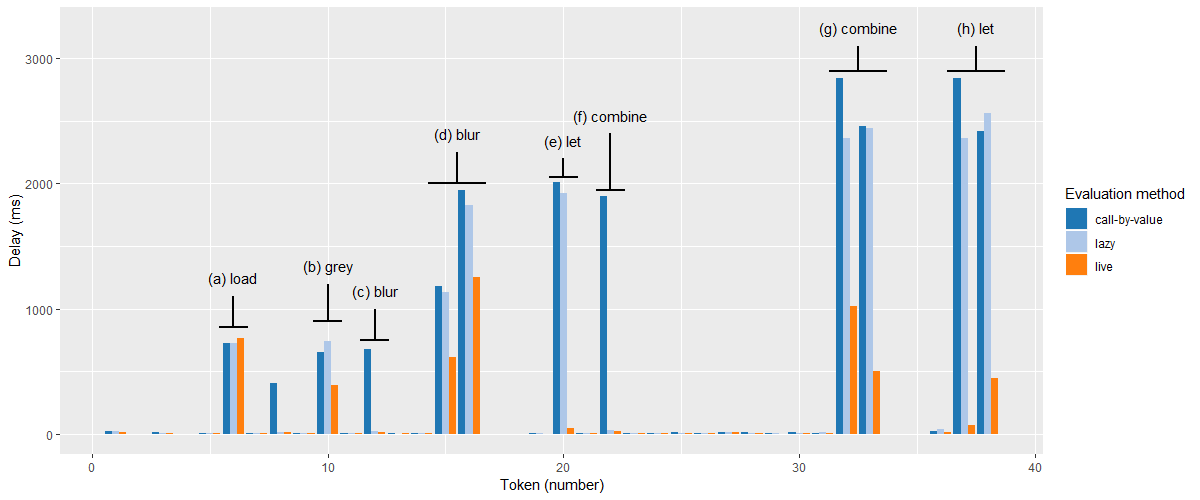
\includegraphics[width=\linewidth]{figures/drawing.png} \end{wide}
\caption{Time required to recompute the results of a sample program after individual tokens
  are added or modified for three different evaluations strategies.}
\label{fig:drawing}
%
\end{figure}

% --------------------------------------------------------------------------------------------------

\begin{figure}
%
\begin{wide}
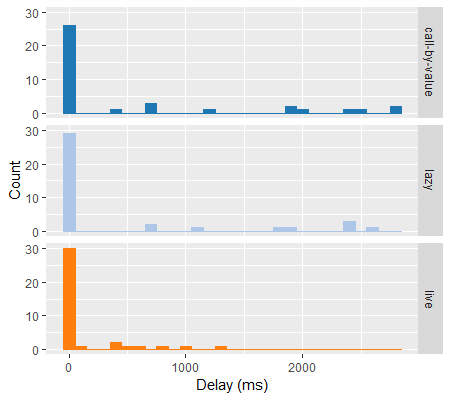
\includegraphics[width=.5\linewidth]{figures/hist-all.png}%
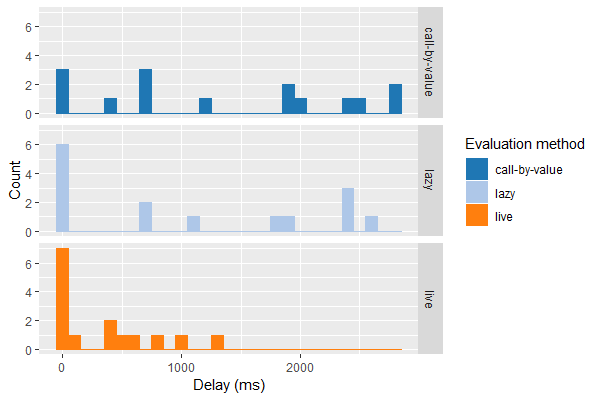
\includegraphics[width=.5\linewidth]{figures/hist-slow.png}
\end{wide}
\caption{Distribution of delays incurred when updating previews.
  We show a histogram computed from all delays (left) and only from delays larger
  than \SI{15}{\ms} (right).}
\label{fig:drawing-hist}
%
\end{figure}

% --------------------------------------------------------------------------------------------------

The experimental environment is implemented in F\# and compiled to JavaScript using the Fable
compiler. We run the experiments in Firefox (version 64.0.2, 32bit) on Windows 10
(build 1809, \SI{64}{\bit}) on Intel Core i7-7660U CPU with \SI{16}{\giga\byte} RAM.

\Cref{fig:drawing} shows times needed to recompute previews after individual tokens
are added, deleted or modified, according to the script in
\cref{fig:image-edits}, resulting in 38 measurements. We mark a number of notable points in the chart:

~

\begin{enumerate}
  \renewcommand{\theenumi}{\alph{enumi}}%
\item Loading image for the first time incurs small extra overhead in the live strategy.
\item Greyscaling using the live strategy does not need to re-load the image.
\item Accessing the blur member without arguments causes delay for call-by-value.
\item When varying the parameter of blur, the live strategy reuses the greyscaled image.
\item Introducing let binding does not cause recomputation when using live strategy.
\item As in (c), accessing a member without an argument only affects call-by-value.
\item The live strategy is much faster when varying the parameter of combine.
\item Introducing let binding, again, causes full recomputation for lazy and call-by-value.
\end{enumerate}
%
%
A summarized view of the delays is provided in \cref{fig:drawing-hist}, which shows
histograms illustrating the distribution of delays for each of the three evaluation methods.
A large proportion of delays is very small (less than \SI{15}{\ms}) because the parser used in our
experimental environment often fails (e.\hairspace g.~for unclosed parentheses). The histogram
on the right summarizes only delays for edit operations where the delay for at least one of
the strategies was over \SI{15}{\ms}. The histogram shows that the live strategy eliminates the longest
delays (by caching partial results), with the exception of a few where the underlying operation
takes a long time (such as blurring the image). The results would be even more significant with
an error-recovering parser.

The purpose of our experiment is not to exactly assess the overhead of our implementation.
Our goal is to illustrate how often can previously evaluated results be reused and the impact
this has when writing code. The experiment presented in this section is small-scale, but it is
sufficient for this purpose. When recomputing results after every edit
using the \emph{call-by-value} strategy, the time needed to update results grows
continually. The \emph{lazy} strategy removes the overhead for programs that fail, but
keeps the same trend. Our \emph{live} strategy reuses values computed
previously. Consequently, expensive operations such as (d) and (g) in \cref{fig:drawing}
are significantly faster, because they do not need to recompute operations done previously when
writing the code. As shown in \cref{fig:drawing-hist}, there are almost no very expensive
operations (taking over 1 second) in the \emph{live} strategy in contrast to several in the
other two strategies.

% --------------------------------------------------------------------------------------------------

\begin{figure}
  \begin{wide}
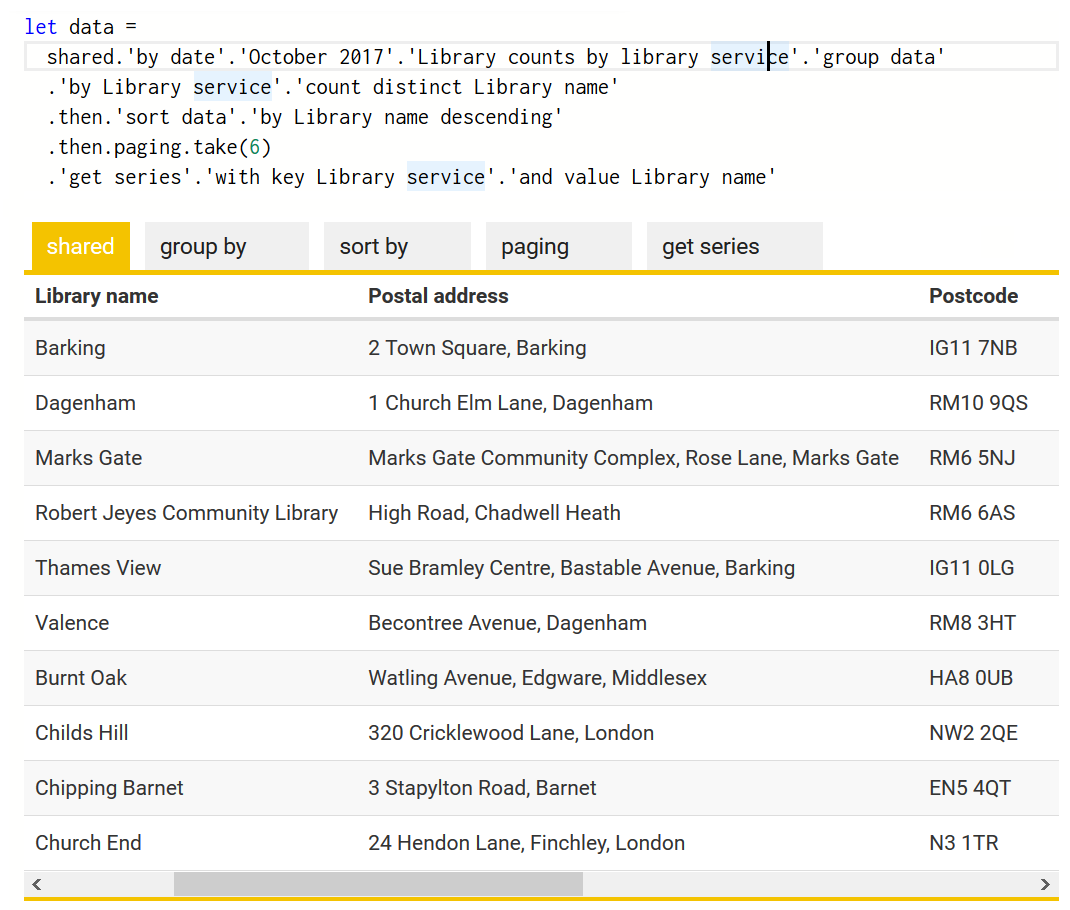
\includegraphics[width=.5\linewidth]{figures/gallery1.png}
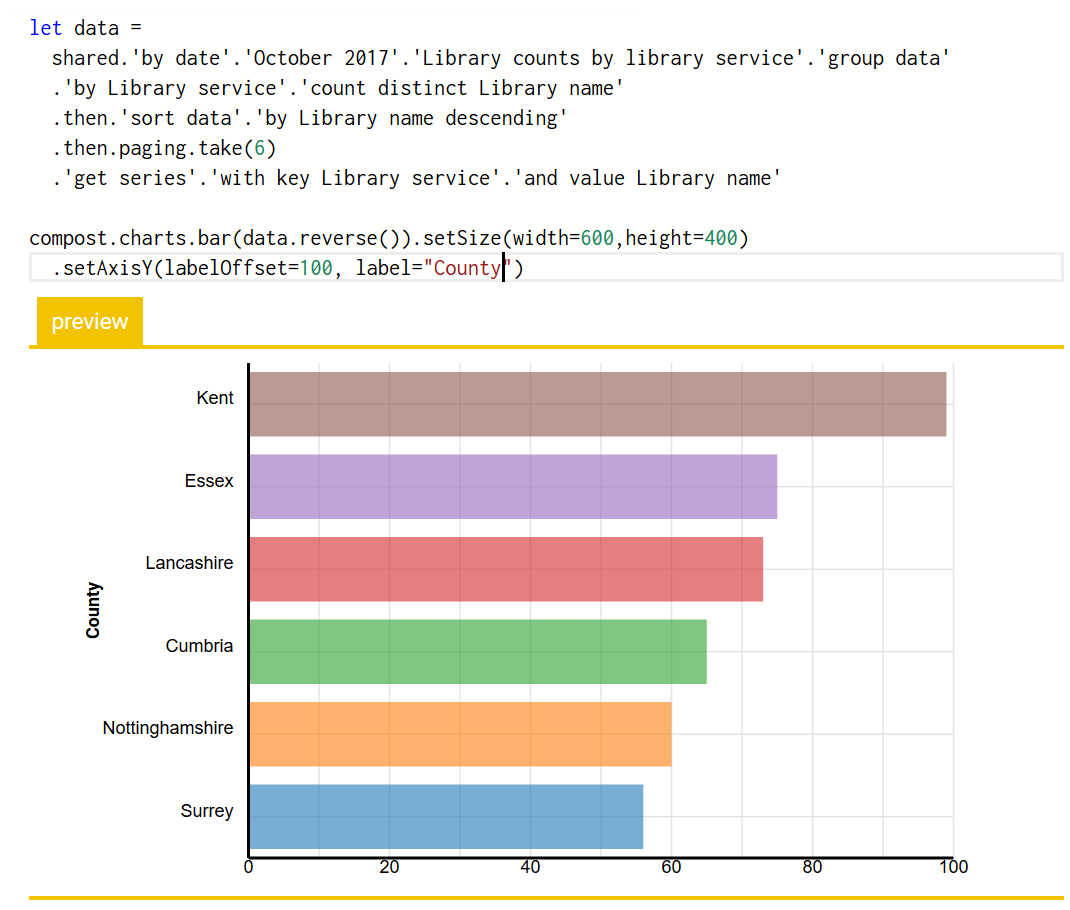
\includegraphics[width=.5\linewidth]{figures/gallery2.png}
\end{wide}
\caption{Data analysis counting the number of libraries per county in the UK. We load
  and aggregate data (left) and then create a chart with a label (right).
  The example has been created using our tool discussed in \cref{sec:evaluation-case}
  by a non-programmer and is available at \url{http://gallery.thegamma.net/73/}.}
\label{fig:gallery}
%
\end{figure}

% --------------------------------------------------------------------------------------------------

\subsection{Transparent tools for data journalism}
\label{sec:evaluation-case}

In \cref{sec:background-jupyter}, we motivated our work by considering how journalists
explore open data. In addition to the theoretical and experimental work presented in this paper,
we also implemented an online data exploration environment, equipped with live editor for The
Gamma language that provides instant feedback during coding. The environment uses the
principles presented in this paper to build a more comprehensive system that allows users,
such as journalists, to analyse, summarize and visualize open data. In this section, we briefly
report on our experience with the system. Two screenshots shown
in \cref{fig:gallery} illustrate a number of interesting features:

\begin{itemize}
\item The left screenshot uses a type provider for data aggregation~\cite{gamma}.
  Type provider are treated as an external library
  (with objects, members and reduction relation). Type providers also rely on type information to
  provide editor auto-complete, which we support by implementing type checking over a
  dependency graph (\cref{sec:extra-types}).

\item When displaying instant preview for code written using the data aggregation type provider (left),
  our environment generates tabes that show individual steps of the data transformation.
  A tab is selected based on the cursor position and shows a preview for the current sub-expression
  (e.\hairspace g.~raw data before grouping).

\item Another external library provides support for charting (right). Here, the environment
  displays the result of evaluating the whole command. The screenshot shows a case where the user
  modifies parameters of the chart. Thanks to our live evaluation
  strategy, this is done efficiently without reevaluating the data transformation.
\end{itemize}
%
%
The environment is available at \url{http://gallery.thegamma.net}.
A user study to evaluate the usability of the system from a human-computer interaction perspective
is left for future work. As an anecdotal evidence, the code in
\cref{fig:gallery} was developed by an attendee of a Mozilla Festival 2017
who had no prior programming experience.


% ==================================================================================================

\section{Related and future work}
\label{sec:future}

Simple data exploration performed, for example, by journalists~\cite{ddj} is done either
programmatically or using spreadsheets. The latter is easy but error-prone while the former
requires expert programming skills. We aim to bring liveness of spreadsheets to programmatic
data exploration. This requires extending recomputation as done in spreadsheets~\cite{spreadsheet}
to code written in an ordinary text editor.

\paragraph{Notebooks and data science tools.}
Visual data exploration tools are interactive~\cite{control,tableau,vizdom} and some
can export the workflow as a script~\cite{wrangler}, but data analysts who prefer code
typically resort to notebook systems such as Jupyter or R Markdown~\cite{jupyter,rmarkdown}.
Those are text-based, but have a limited model of recomputation. Users structure code in
cells and manually reevaluate cells. Many notebook systems are based on the REPL (read-eval-print-loop)%
~\cite{lisp,drscheme} and do not track dependencies between cells, which can lead to well-documented
inconsistencies~\cite{dataflow,noworkflow,wrattler}.

Ideas such as dependency tracking and efficient recomputation exist in visual data exploration tools%
~\cite{control,tableau,vizdom} and scientific workflow systems~\cite{taverna,kepler}. The
implementation techniques are related to our work, but we focus on text-based scripts.
Tempe~\cite{tempe} focuses on streaming data, but provides a text-based scripting environment
with automatic code update; its usability in contrast to REPLs has been empirically
evaluated~\cite{ripple}.

\paragraph{Live and exploratory programming.}
Live programming based on textual programs has been popularised by \citeauthor{learnable}~\cite{learnable,principle} and
is actively developed in domains such as live coded music~\cite{beyond,sonic}.
The notions of exploratory and live programming have been extensively studied~\cite{review}.
The notion of exploratory programming has recently been analysed from the perspective of
human-computer interaction \cite{exploratory}, which led to new tools~\cite{variolite},
complementary to our instant previews. \Citeauthor{liveroad}~\cite{liveroad}
review the use of live programming in a Smalltalk derived environment. Lighttable~\cite{lighttable}
and Chrome DevTools provide limited instant previews akin to those presented in this paper,
but without well specified recomputation model. Finally, work on keeping state during
code edits~\cite{alive,livingit} would be relevant for supporting streaming data.

A more principled approach can be used by systems based on structured editing~\cite{structure-based,interactive,livenut,lamdu}
where code is only modified via known operations with known effect on the computation graph
(e.\hairspace g.~``extract variable'' has no effect on the result; ``change constant value''
forces recomputation of subsequent code). This can be elegantly implemented using bi-directional
lambda calculus~\cite{hazelnut}, but it also makes us consider more human-centric abstractions%
~\cite{subtext,directprog} further discussed in \cref{sec:extra-abstraction}.

\paragraph{Incremental computation and dependency analysis.}
Work on self-adjusting and incremental computation~\cite{selfadjusting,adapton} handles
recomputation when the program stays the same, but input changes.
Most incremental systems, e.\hairspace g.~\cite{incremental,adaptivefp,deltaml} evaluate the program and use
programmer-supplied information to build a dependency graph, whereas our system uses static code analysis;%
\cite{adapton} implement a small adaptive interpreter
that treats code as changing input data, suggesting an implementation technique for
live programming systems. Our use of dependency graphs~\cite{dependencies} is static and first-order
and can be seen as a form of program slicing~\cite{slicing}, although our binding process is
more directly inspired by Roslyn~\cite{roslyn}, which uses it for efficient background type-checking.

\paragraph{Semantics and partial evaluation.}
The evaluation of previews is a form of partial evaluation~\cite{partial}, done in a
way that allows caching. This can be done implicitly or explicitly in the form of
multi-stage programming~\cite{metaml}. Semantically, the evaluation of previews can be seen as a
modality and delayed previews are linked to contextual modal type theory~\cite{cmtt},
formally modelled using comonads~\cite{cmtt-denotation}.



% ==================================================================================================
%
\section{Summary}
One of the aspects that make spreadsheets easier to use than programming tools is that they
provide instant feedback. We aim to make programming tools as instant as spreadsheets.
We described a number of key aspects of simple data analyses such as those done by journalists
and then used our observations to build both theory and simple practical data analytics tools.

Our \emph{data exploration calculus} is a simple formally tractable language
for data exploration. The calculus captures key observations about simple data analyses. They
rely on logic defined by external libraries, implement few abstractions and are written as lists of
commands.

Our main technical contribution is a \emph{instant preview} mechanism that efficiently evaluates
code during editing and instantly provides a preview of the result. We allow users to edit code
in unconstrained way in an text editor, which makes this particularly challenging. The key trick
is to separate the process into a fast \emph{binding phase}, which constructs a dependency graph
and a slower \emph{evaluation phase} that can cache results. This makes it possible to quickly parse
updated code, reconstruct dependency graph and compute preview using previous, partially
evaluated, results.

We evaluated our approach in three ways. First, we proved that our mechanism is correct and
that it reuses evaluated values for many common code edit operations. Second, we conducted an
experimental study that illustrates how often are previously evaluated results reused during
typical programming scenario. Thirdly, we used our research as a basis for online data exploration
environment, which shows the practical usability of our work.

\acks
\begin{sloppypar}
 We thank Dominic Orchard, Stephen Kell, Roly Perera and Jonathan
  Edwards for many discussions about the work presented in the paper. Dominic
  Orchard provided invaluable feedback on earlier version of the paper. The
  paper also benefited from suggestions made by anonymous reviewers of The
  Programming Journal as well as reviwers of earlier versions of the paper.
  This work was partly supported by The Alan Turing Institute under the EPSRC
  grant EP/N510129/1.
\end{sloppypar}
% ==================================================================================================

\printbibliography

% ==================================================================================================

\appendix

\section{Details of proofs}

\subsection{Normalization for data exploration calculus}
\label{sec:app-normalization}

\begin{theorem}[Normalization]
For all $p$, there exists $n$ and $o_1, \ldots, o_n$ \\
such that $p\rightsquigarrow^{*} o_1;\ldots;o_n$.
\end{theorem}
\begin{proof}
We define $\ident{size}$ of a program in data exploration calculus as follows:
\begin{equation}
\begin{array}{rcl}
\ident{size}(c_1; \ldots; c_n) &=& 1 + \Sigma^{n}_{i=1} \ident{size}(c_i)\\
\ident{size}(\kvd{let}~x=t) &=& 1 + \ident{size}(t)\\
\ident{size}(e_0.m(e_1, \ldots, e_n)) &=& 1 + \Sigma^{n}_{i=0} \ident{size}(e_i)\\
\ident{size}(\lambda x\rightarrow e) &=& 1 + \ident{size}(e)\\
\ident{size}(o) = \ident{size}(x) &=& 1\\
\end{array}
\end{equation}
%
%
The property holds because, first, both \rname{let} and \rname{external} decrease the \ident{size}
of the program and, second, a program is either fully evaluated, i.\hairspace e.~$o_1;\ldots;o_n$ for some $n$
or, it can be reduced using one of the reduction rules.
\end{proof}


\subsection{Let elimmination for a program}
\label{sec:let-lang-elimination}

\begin{lem}[Let elimination for a program]
\label{thm:let-lang-elimination-proof}
Given any program $p$ such that $p \rightsquigarrow^{*} o_1;\ldots;o_n$ for some $n$ and $o_1, \ldots, o_n$
then if $p \rightsquigarrow_\ident{let} p'$ for some $p'$ then also $p' \rightsquigarrow^{*} o_1;\ldots;o_n$.
\end{lem}
\begin{proof}
The elimination of let binding transforms a program $c_1;\; \ldots;\; c_{k-1};\; \kvd{let}~x=t;\; c_{k+1};\; \ldots; c_n$
to a program $c_1;\; \ldots;\; c_{k-1};\; t; c_{k+1}[x\leftarrow t];\; \ldots; c_n[x\leftarrow t]$.
The reduction steps for the new program can be constructed using the steps of $p \rightsquigarrow^{*} o_1;\ldots;o_n$.
The new command $t$ reduces to an object $o$ using the same steps as the original term $t$
in $\kvd{let}~x=t$ but with context $C_c = -$ rather than $C_c = \kvd{let}~x=-$; the terms $t$
introduced by substitution also reduce using the same steps as before, but using
contexts in which the variable $x$ originally appeared.
\end{proof}

\subsection{Let elimination for a dependency graph}
\label{sec:app-let-grp-elimination}

\begin{lem}[Let elimintion for a dependency graph]
\label{thm:app-let-grp-elimination}
Given programs $p_1, p_2$ such that $p_1 \rightsquigarrow_\ident{let} p_2$ and a lookup table
$\Delta_0$ then if $\bndclr{v_1}; \ldots; \bndclr{v_n}, (V, E) = \ident{bind-prog}_{\emptyset, \Delta_0}(p_1)$ and
$\bndclr{v'_1};\ldots;\bndclr{v'_n}, (V', E') = \ident{bind-prog}_{\emptyset, \Delta_1}(p_2)$ such that $\Delta_1 = \ident{update}_{V, E}(\Delta_0)$
then for all $i$, $\bndclr{v_i} = \bndclr{v'_i}$ and also $(V, E) = (V', E')$.
\end{lem}
\begin{proof}
Assume $p_1 = c_1; \ldots; c_{k-1}; \kvd{let}~x=e; c_{k+1};\ldots; c_n$ and the let binding is
eliminated resulting in $p_2 = c_1; \ldots; c_{k-1}; e; c_{k+1}[x\leftarrow e];\ldots; c_n[x\leftarrow e]$.
When binding $p_1$, the case $\ident{bind-prog}_{\Gamma,\Delta}(\kvd{let}~x=e)$ is handled using (7)
and the node resulting from binding $e$ is added to the graph $V, E$. It is then referenced each
time $x$ appears in subsequent commands $c_{k+1}; \ldots; c_n$.
When binding $p_2$, the node resulting from binding $e$ is a primitive value or a node already
present in $\Delta_1$ (added by $\ident{update}_{V, E}$) and is reused each time
$\ident{bind-expr}_{\Gamma,\Delta_1}(e)$ is called.
\end{proof}


\subsection{Term preview correctness}
\label{sec:app-correctness}

\begin{theorem}[Term preview correctness]
Given a term $t$ that has no free variables, together with a lookup table $\Delta$ obtained
from any sequence of programs using $\ident{bind-prog}$ (\cref{fig:binding-rules-prog}) and
$\ident{update}$ (\cref{fig:loop}), then
let $\bndclr{v}, (V, E) = \ident{bind-expr}_{\emptyset, \Delta}(t)$. If $\bndclr{v}\Downarrow p$
over a graph $(V, E)$ then $p = o$ for some value $o$ and $t \rightsquigarrow^{*} o$.
\end{theorem}

\begin{proof}
When combining recursively constructed sub-graphs, the \ident{bind-expr} function
adds new nodes and edges leading from those new nodes. Therefore, an evaluation using~$\Downarrow$
over a sub-graph will also be valid over the new graph -- the newly added nodes and edges do not introduce
non-determinism to the rules given in \cref{fig:eval}.

We prove a more general property showing that for any $e$, its binding
$\bndclr{v}, (V, E) = \ident{bind-expr}_{\emptyset, \Delta}(e)$ and any evaluation context $C$
such that $C[e]\rightsquigarrow o$ for some $o$, one of the following holds:
%
\begin{enumerate}
  \renewcommand{\theenumi}{\alph{enumi}}%
\item If $FV(e)\,=\,\emptyset$ then $\bndclr{v} \Downarrow p$ for some $p$ and $C[p] \rightsquigarrow o$
\item If $FV(e)\neq\emptyset$ then $\bndclr{v} \Downarrow \llbracket e_p \rrbracket_{FV(e)}$ for some $e_p$ and $C[e_p] \rightsquigarrow o$
\end{enumerate}
%
In the first case, $p$ is a value, but it is not always the case that $e \rightsquigarrow^{*} p$,
because $p$ may be lambda function and preview evaluation may reduce sub-expression in the body of
the function. Using a context $C$ in which the value reduces to an object avoids this problem.

The proof of the theorem follows from the more general property. Using a context $C[-]=-$, the
term $t$ reduces $t \rightsquigarrow^{*}t' \rightsquigarrow_\epsilon o$ for some $o$ and the
preview $p$ is a value $o$ because $C[p] = p = o$.
The proof is by induction over the binding process, which follows the structure of the expression:

\begin{enumerate}
  \renewcommand*\labelenumi{\usekomafont{listlabel}\theenumi}
  \renewcommand{\theenumi}{(\arabic{enumi})}%

\item \label{itm:1} $\ident{bind-expr}_{\Gamma, \Delta}(e_0.m(e_1, \ldots, e_n))$ --
  Here $e = e_0.m(e_1, \ldots, e_n)$, $\bndclr{v_i}$ are graph nodes obtained by induction for
  expressions $e_i$ and $\{ (\bndclr{v}, \bndclr{v_0}, \blbl{arg}(0)), \ldots, (\bndclr{v}, \bndclr{v_n}, \blbl{arg}(n))\} \subseteq E$.
  From lookup inversion \cref{thm:lemma-lookup}, $\bndclr{v} = \bnd{mem}(m, s)$ for some $s$.

  If $FV(e)=\emptyset$, then $\bndclr{v_i} \Downarrow p_i$ for $i\in 0\ldots n$ and
  $\bndclr{v}\Downarrow p$ using \rname{mem-val} such that $p_0.m(p_1, \ldots, p_n) \rightsquigarrow p$.
  From induction hypothesis and \emph{compositionality} of external libraries (\cref{def:external}),
  it holds that for any $C$ such that $C[e_0.m(e_1, \ldots, e_n)] \rightsquigarrow o$ for some $o$
  then also $C[p_0.m(p_1, \ldots, p_n)] \rightsquigarrow C[p] \rightsquigarrow o$.

  If $FV(e)\neq\emptyset$, then $\bndclr{v_i} \Downarrow_\ident{lift} \llbracket e'_i \rrbracket$ for $i\in 0\ldots n$ and
  $\bndclr{v}\Downarrow \llbracket e'_0.m(e'_1, \ldots, e'_n) \rrbracket_{FV(e)}$ using \rname{mem-expr}.
  From induction hypothesis and \emph{compositionality} of external libraries (\cref{def:external}),
  it holds that for any $C$ such that $C[e_0.m(e_1, \ldots, e_n)] \rightsquigarrow o$ for some $o$
  then also $C[e'_0.m(e'_1, \ldots, e'_n)] \rightsquigarrow o$.

\item  $\ident{bind-expr}_{\Gamma, \Delta}(e_0.m(e_1, \ldots, e_n))$ --
  This case is similar to \labelcref{itm:1}, except that the fact that $\bndclr{v} = \bnd{mem}(m, s)$
  holds by construction, rather than using \cref{thm:lemma-lookup}.

\item \label{itm:3} $\ident{bind-expr}_{\Gamma, \Delta}(\lambda x\rightarrow e_b)$ --
  Here $e = \lambda x\rightarrow e_b$, $\bndclr{v_b}$ is the graph node obtained by induction
  for the expression $e_b$ and $(\bndclr{v}, \bndclr{v_b}, \blbl{body}) \in E$.
  From lookup inversion \cref{thm:lemma-lookup}, $\bndclr{v} = \bnd{fun}(x, s)$ for some $s$.
  The evaluation can use one of three rules:

  \begin{enumerate}
    \renewcommand{\theenumii}{\roman{enumii}}%
  \item
  If $FV(e)=\emptyset$ then $\bndclr{v_b}\Downarrow p_b$ for some $p_b$ and $\bndclr{v}\Downarrow \lambda x\rightarrow p_b$
  using \rname{fun-val}. Let $e'_b=p_b$.

  \item
  If $FV(e_b)=\{x\}$ then $\bndclr{v_b}\Downarrow \llbracket e'_b \rrbracket_x$ for some $e'_b$ and
  $\bndclr{v}\Downarrow \lambda x\rightarrow e'_b$ using \rname{fun-bind}.

  \item
  Otherwise, $\bndclr{v_b}\Downarrow \llbracket e'_b \rrbracket_{x,\Gamma}$ for some $e'_b$ and
  $\bndclr{v}\Downarrow \llbracket\lambda x\rightarrow e'_b\rrbracket_\Gamma$ using \rname{fun-expr}.
  \end{enumerate}
%
%
For i.) and ii.) we show that a.) is the case; for iii.) we show that b.) is the case; that is
for any $C$, if $C[\lambda x\rightarrow e_b] \rightsquigarrow o$ then also
$C[\lambda x\rightarrow e'_b] \rightsquigarrow o$. For a given $C$, let $C'[-] = C[\lambda x\rightarrow -]$
and use the induction hypothesis, i.\hairspace e.~if $C'[e_b] \rightsquigarrow o$ for some $o$ then also $C'[e'_b] \rightsquigarrow o$.

\item \label{itm:4} $\ident{bind-expr}_{\Gamma, \Delta}(\lambda x\rightarrow e)$  --
  This case is similar to \labelcref{itm:3}, except that the fact that $\bndclr{v} = \bnd{fun}(x, s)$
  holds by construction, rather than using \cref{thm:lemma-lookup}.

\item $\ident{bind-expr}_{\Gamma, \Delta}(o)$ -- In this case $e=o$ and $\bndclr{v} = \bnd{val}(o)$
  and $\bnd{val}(o)\Downarrow o$ using \rname{val} and so the case a.) trivially holds.

\item $\ident{bind-expr}_{\Gamma, \Delta}(x)$ -- The initial $\Gamma$ is empty,
  so $x$ must have been added to $\Gamma$ by case \labelcref{itm:3} or \labelcref{itm:4}. Hence,
  $\bndclr{v}=\bnd{var}(x)$, $\bndclr{v}\Downarrow \llbracket x \rrbracket_{x}$ using \rname{var}
  and so $e_p = e = x$ and the case b.) trivially holds.
\end{enumerate}
\end{proof}

\subsection{Binding sub-expressions}
\label{sec:sub-expr}

\begin{lem}[Binding sub-expressions]
\label{thm:sub-expr}
Assume we have programs $p_1, p_2$ such that $p_1 = c_1; \ldots; c_k; K_c[e]; c_{k+1};\ldots; c_n$ and
$p_2 = c'_1; \ldots; c'_k; K'_c[e]; c'_{k+1};\ldots;c'_n$ and $I\subseteq \{1\ldots k\}$ such
that $\forall i\!\in\!I.\,c_i\!=\!c'_i$ and for each $x \in \bigcup_{i\in I}FV(c_i) \cup FV(e)$
there exists $j\in I$ such that $c_j = \kvd{let}\,x=e$ for some $e$.
%
Given any $\Delta$, assume that the the first program is bound,
i.\hairspace e.~$\bndclr{v_1};\ldots;\bndclr{v_n}, (V, E) = \ident{bind-prog}_{\emptyset, \Delta}(p_1)$,
the cache is updated $\Delta' = \ident{update}_{V, E}(\Delta)$ and the second
program is bound,
i.\hairspace e.~$\bndclr{v'_1};\ldots;\bndclr{v'_n}, (V', E') = \ident{bind-prog}_{\emptyset, \Delta'}(p_2)$.

Now, assume $\bndclr{v}, G = \ident{bind-expr}_{\Gamma, \Delta}(e)$ and
$\bndclr{v'}, G' = \ident{bind-expr}_{\Gamma', \Delta'}(e)$ are the recursive calls to bind
$e$ during the first and the second binding, respectively. Then, the graph nodes assigned to the
sub-expression $e$ are the same, i.\hairspace e.~$\bndclr{v} = \bndclr{v'}$.
\end{lem}
\begin{proof}
First, assuming that $\forall x\in FV(e). \Gamma(x) = \Gamma'(x)$, we show by induction over the binding process of $e$
for the first program that the result is the same. In cases (1) and (3), the updated $\Delta'$
contains the required key and so the second binding proceeds using the same case. In cases
(2) and (4), the second binding reuses the node created by the first binding using case (1) and
(3), respectively. Cases (5) and (6) are the same.

Second, when binding let bindings in $c_1; \ldots; c_k$, the initial $\Gamma = \emptyset$ during
both bindings. Nodes added to $\Gamma$ and $\Gamma'$ for commands $c_j$ such that $j\in I$ are
the same and nodes added for remaining commands do not add any new nodes referenced from $e$ and
so $\bndclr{v} = \bndclr{v'}$ using the above.
\end{proof}


% ==================================================================================================

\section{Theories of delayed previews}
\label{sec:app-theories}

The operational semantics presented in this paper serves two purposes. It gives a simple guide
for implementing text-based live programming environments for data science and we use it to prove that
our optimized way of producing instant previews is correct. However, some aspects of our mechanism
are related to important work in semantics of programming languages and deserve to be mentioned.

The construction of delayed previews is related to meta-programming. Assuming
we have delayed previews $\llbracket e_0 \rrbracket_x$ and $\llbracket e_1 \rrbracket_y$ and
we invoke a member $m$ on $e_0$ using $e_1$ as an argument. To do this, we construct a new
delayed preview $\llbracket e_0.m(e_1) \rrbracket_{x, y}$. This operation is akin to expression
splicing from meta-programming~\cite{metaml,quotations}.

The semantics of delayed previews can be more formally captured by Contextual Modal Type Theory
(CMTT)~\cite{cmtt} and comonads~\cite{cmtt-denotation}. In CMTT, $\lbrack \Psi \rbrack A$ denotes
that a proposition $A$ is valid in context $\Psi$, which is similar to our delayed previews written
as $\llbracket A \rrbracket_\Psi$. CMTT defines rules for composing context-dependent propositions
that would allow us to express the splicing operation used in \rname{mem-expr}. In categorical
terms, the context-dependent proposition can be modelled as a graded comonad~\cite{effectrev,graded}.
The evaluation of a preview with no context dependencies (built implicitly into our evaluation rules)
corresponds to the counit operation of a comonad and would be explicitly written as
$\llbracket A \rrbracket_\emptyset \rightarrow A$.

% ==================================================================================================

\begin{figure}
\vspace{-0.5em}
\begin{equation*}
\hspace{3em}
\xymatrix{
\bnd{mem}(m, s_0) \ar@/_1pc/[drr]_{\blbl{arg}(1)} \ar[rr]^{\blbl{arg}(0)} && \bnd{val}(o) && \bnd{var}(x, s_1)\ar[ll]_{\blbl{callsite}(m, 1)} \\
&&\bnd{fun}(x, s_2) \ar[u]_{\blbl{callsite}(m, 1)} \ar@/_1pc/[rru]_{\blbl{body}} &&
}
\end{equation*}
\vspace{-0.5em}
\caption{Dependency graph for $o.m(\lambda x\rightarrow x)$ with a newly added \blbl{callsite} edges.}
\label{fig:graph-func}
\vspace{-0.5em}
\end{figure}

% --------------------------------------------------------------------------------------------------

\section{Type checking}
\label{sec:extra-types}

Instant previews give analysts quick feedback when they write incorrect code, but
having type information is still valuable. First, it can help give better error messages. Second,
types can be used to provide auto-complete -- when the user types `.' we can offer available
members without having to wait until the value of the object is available.

\paragraph{Revised dependency graph.}
Type checking of small programs is typically fast enough that no caching is necessary. However,
The Gamma supports \emph{type providers}~\cite{providers-fsharp,providers-idris}, which can
generate types based on an external file or a REST service call, e.\hairspace g.~\cite{fsdata}. For this
reason, type checking can be relatively time consuming and can benefit from the same caching
facilities as those available for instant previews.

Adding type checking requires revising the way we construct the dependency graph introduced in
\cref{sec:formal}. Previously, a variable bound by a lambda function had no dependencies.
However, the type of the variable depends on the context in which it appears. Given an expression
$o.m(\lambda x\rightarrow x)$, we infer the type of $x$ from the type of the first argument
of the member $m$. A variable node for $x$ thus needs to depend on the call site of $m$.
We capture that by adding an edge $\blbl{callsite}(m, i)$ from $x$ to $o$ which indicates that
$x$ is the input variable of a function passes as the $i^\textnormal{th}$ argument to the $m$
member of the expression represented by the target node. We also add $\blbl{callsite}(m, i)$
as an edge from the node of the function. \Cref{fig:graph-func} shows the
revised dependency graph for $o.m(\lambda x\rightarrow x)$. %A revised version of the algorithm
%that constructs the dependency graph is included in \cref{sec:app-types}.

\paragraph{Type checking.}
The structure of typing rules is similar to the evaluation relation $\bndclr{v}\Downarrow d$
defined earlier. Given a dependency graph $(V, E)$, we define typing judgements in the form
$\bndclr{v}\vdash \tau$. The type $\tau$ can be a primitive type, a function $\tau \rightarrow \tau$
or an object type $\{m_1\!:\!\sigma_1, \ldots, m_n\!:\!\sigma_n\}$ with member types
$\sigma = (\tau_1, \ldots, \tau_n) \rightarrow \tau$.

The typing rules for variables, functions and member access are shown in \cref{fig:tc}.
%Remaining rules are available in \cref{sec:app-types}.
When type checking a member access \rname{mem}, we find its dependencies $\bndclr{v_i}$ and
check that the instance is an object with the required member $m$. The types of arguments of the
member then need to match the types of the remaining (non-instance) nodes.
Type checking a function \rname{fun} and a variable \rname{var} is similar. In both cases,
we follow the \blbl{callsite} edge to find the member that accepts the function as an argument
and use the type of the argument to check the type of the function or infer the type of the
variable.

The results of type checking can be cached and reused in the same way as instant previews, although
we leave out the details. A property akin to correctness (\cref{thm:correcntess})
requires defining standard type checking over the structure of expressions, which we also
omit for space reasons.

% --------------------------------------------------------------------------------------------------

\begin{figure}
\begin{equation*}
\hspace{-1em}
\begin{array}{l}
\hspace{7em}\inference[\rname{var}~]
  { (\bnd{var}(x,s), \bndclr{v}, \blbl{callsite}(m, i)) \in E \\
    \bndclr{v} \vdash \{.., m:(\tau_1, \ldots, \tau_k)\rightarrow \tau,..\} & \tau_i=\tau'\rightarrow\tau'' }
  { \bnd{var}(x, s) \vdash \tau' }
\\[1.5em]
\hspace{7em}\inference[\rname{mem}~]
  { \forall i\in\{0\ldots k\}.(\bnd{mem}(m, s), \bndclr{v_i}, \blbl{arg}(i)) \in E \\
  \bndclr{v_0} \vdash \{.., m:(\tau_1, \ldots, \tau_k) \rightarrow \tau, ..\} & \bndclr{v_i} \vdash \tau_i }
  { \bnd{mem}(m, s) \vdash \tau }
\\[1.5em]
\hspace{4em}\inference[\rname{fun}~]
  { \{(\bnd{fun}(x,s), \bndclr{v_b}, \blbl{body}), (\bnd{var}(x,s), \bndclr{v_c}, \blbl{callsite}(m, i))\} \subseteq E \\
    \bndclr{v_c} \vdash \{.., m:(\tau_1, \ldots, \tau_k)\rightarrow \tau,..\} &
    \tau_i=\tau'\rightarrow\tau'' & \bndclr{v_b} \vdash \tau'' }
  { \bnd{fun}(x, s) \vdash \tau' \rightarrow \tau'' }
\end{array}
\end{equation*}
\vspace{-0.5em}
\caption{Rules that define type checking of terms and expressions over a dependency graph $(V, E)$}
\label{fig:tc}
\vspace{-0.5em}
\end{figure}

% --------------------------------------------------------------------------------------------------

\section{Feedback-friendly abstraction}
\label{sec:extra-abstraction}

The data analysis by Financial Times in \cref{sec:background-jupyter} illustrates why
notebook users often avoid abstraction. Wrapping code in a function makes it impossible to
split code into cells and see results of intermediate steps. Instead, the analysis used a
global variable with possible values in a comment.

Providing instant previews inside ordinary functions is problematic, because we do not have readily
available values for input parameters and our mechanism for lambda functions only provides
delayed previews inside body of a function. We believe that extending the data exploration calculus
with an abstraction mechanism that would support development with instant feedback is an
interesting design problem and we briefly outline a possible solution here.

Data scientists often write code interactively using a sample data set and, when it works well,
wrap it into a function that they then call on other data. Similarly, spreadsheet users
often write equation in the first row of a table and then use the ``drag down'' operation to
apply it to other rows. One way of adding similar functionality to the data exploration calculus
is to label a sequence of commands such that the sequence can be reused later with different
inputs:
%
\begin{equation*}
\begin{array}{rcl}
p &=& c_1; \ldots; c_n\\
c &=& \kvd{let}\,x=t \lsep t \lsep \textit{lbl}\!:\,p \lsep \textit{lbl}
\end{array}
\end{equation*}
%
%
We introduce two new kinds of commands: a labelled sequence of commands and a reference to a label.
When evaluating, the command $\textit{lbl}$ is replaced with the associated sequence of
commands $p$ before any other reductions. Consequently, variables used in the labelled block are
dynamically scoped and we can use let binding to redefine a value of a variable before invoking
the block repeatedly. The correct use of dynamic scoping can be checked using
coeffects~\cite{coeffects}.

This minimalistic abstraction mechanism supports code reuse without affecting how instant previews
are computed. Commands in a labelled block require variables to be defined before the block.
Those define sample data for development and can be redefined before reusing the block. We
intend to implement this mechanism in a future version of our data
exploration environment (\cref{sec:evaluation-case}).

% ==================================================================================================

\end{document}
